% Options for packages loaded elsewhere
\PassOptionsToPackage{unicode}{hyperref}
\PassOptionsToPackage{hyphens}{url}
%
\documentclass[
]{article}
\usepackage{amsmath,amssymb}
\usepackage{iftex}
\ifPDFTeX
  \usepackage[T1]{fontenc}
  \usepackage[utf8]{inputenc}
  \usepackage{textcomp} % provide euro and other symbols
\else % if luatex or xetex
  \usepackage{unicode-math} % this also loads fontspec
  \defaultfontfeatures{Scale=MatchLowercase}
  \defaultfontfeatures[\rmfamily]{Ligatures=TeX,Scale=1}
\fi
\ifPDFTeX
  \usepackage{lmodern}
\else
  \setmainfont{DejaVu Serif}
  \setsansfont{DejaVu Sans}
  \setmonofont{DejaVu Sans Mono}
  \setmathfont{Latin Modern Math}
\fi
% Use upquote if available, for straight quotes in verbatim environments
\IfFileExists{upquote.sty}{\usepackage{upquote}}{}
\IfFileExists{microtype.sty}{% use microtype if available
  \usepackage[]{microtype}
  \UseMicrotypeSet[protrusion]{basicmath} % disable protrusion for tt fonts
}{}
\makeatletter
\@ifundefined{KOMAClassName}{% if non-KOMA class
  \IfFileExists{parskip.sty}{%
    \usepackage{parskip}
  }{% else
    \setlength{\parindent}{0pt}
    \setlength{\parskip}{6pt plus 2pt minus 1pt}}
}{% if KOMA class
  \KOMAoptions{parskip=half}}
\makeatother
\usepackage{xcolor}
\usepackage{longtable,booktabs,array}
\usepackage{calc} % for calculating minipage widths
% Correct order of tables after \paragraph or \subparagraph
\usepackage{etoolbox}
\makeatletter
\patchcmd\longtable{\par}{\if@noskipsec\mbox{}\fi\par}{}{}
\makeatother
% Allow footnotes in longtable head/foot
\IfFileExists{footnotehyper.sty}{\usepackage{footnotehyper}}{\usepackage{footnote}}
\makesavenoteenv{longtable}
\usepackage{graphicx}
\makeatletter
\def\maxwidth{\ifdim\Gin@nat@width>\linewidth\linewidth\else\Gin@nat@width\fi}
\def\maxheight{\ifdim\Gin@nat@height>\textheight\textheight\else\Gin@nat@height\fi}
\makeatother
% Scale images if necessary, so that they will not overflow the page
% margins by default, and it is still possible to overwrite the defaults
% using explicit options in \includegraphics[width, height, ...]{}
\setkeys{Gin}{width=\maxwidth,height=\maxheight,keepaspectratio}
% Set default figure placement to htbp
\makeatletter
\def\fps@figure{htbp}
\makeatother
\ifLuaTeX
  \usepackage{luacolor}
  \usepackage[soul]{lua-ul}
\else
  \usepackage{soul}
\fi
\setlength{\emergencystretch}{3em} % prevent overfull lines
\providecommand{\tightlist}{%
  \setlength{\itemsep}{0pt}\setlength{\parskip}{0pt}}
\setcounter{secnumdepth}{-\maxdimen} % remove section numbering
\ifLuaTeX
  \usepackage{selnolig}  % disable illegal ligatures
\fi
\IfFileExists{bookmark.sty}{\usepackage{bookmark}}{\usepackage{hyperref}}
\IfFileExists{xurl.sty}{\usepackage{xurl}}{} % add URL line breaks if available
\urlstyle{same}
\hypersetup{
  hidelinks,
  pdfcreator={LaTeX via pandoc}}

\author{}
\date{}

\begin{document}

{
\setcounter{tocdepth}{3}
\tableofcontents
}
\begin{longtable}[]{@{}
  >{\raggedright\arraybackslash}p{(\columnwidth - 0\tabcolsep) * \real{1.0000}}@{}}
\toprule\noalign{}
\endhead
\bottomrule\noalign{}
\endlastfoot
\textbf{PUBLIC-SOURCE RESEARCH BRIEF}

\textbf{Advanced C\textsubscript{n}² Modeling}

\textbf{for High-Energy Laser Atmospheric Effects}

Scientific viability · research landscape · datasets · proposed
Strata-OT neural architecture · model-family roadmap · publication
platform \\
\end{longtable}

\begin{longtable}[]{@{}
  >{\raggedright\arraybackslash}p{(\columnwidth - 2\tabcolsep) * \real{0.0218}}
  >{\raggedright\arraybackslash}p{(\columnwidth - 2\tabcolsep) * \real{0.9782}}@{}}
\toprule\noalign{}
\endhead
\bottomrule\noalign{}
\endlastfoot
& \textbf{BOTTOM LINE}

Proceed---but treat this as a data-and-validation program with a model
at its center. A 20--120M-parameter physics-constrained profile model is
a credible first publication target; a billion-parameter ``foundation
model'' is not justified until the direct-observation corpus is much
larger and more diverse. \\
\end{longtable}

\begin{longtable}[]{@{}
  >{\raggedright\arraybackslash}p{(\columnwidth - 0\tabcolsep) * \real{1.0000}}@{}}
\toprule\noalign{}
\endhead
\bottomrule\noalign{}
\endlastfoot
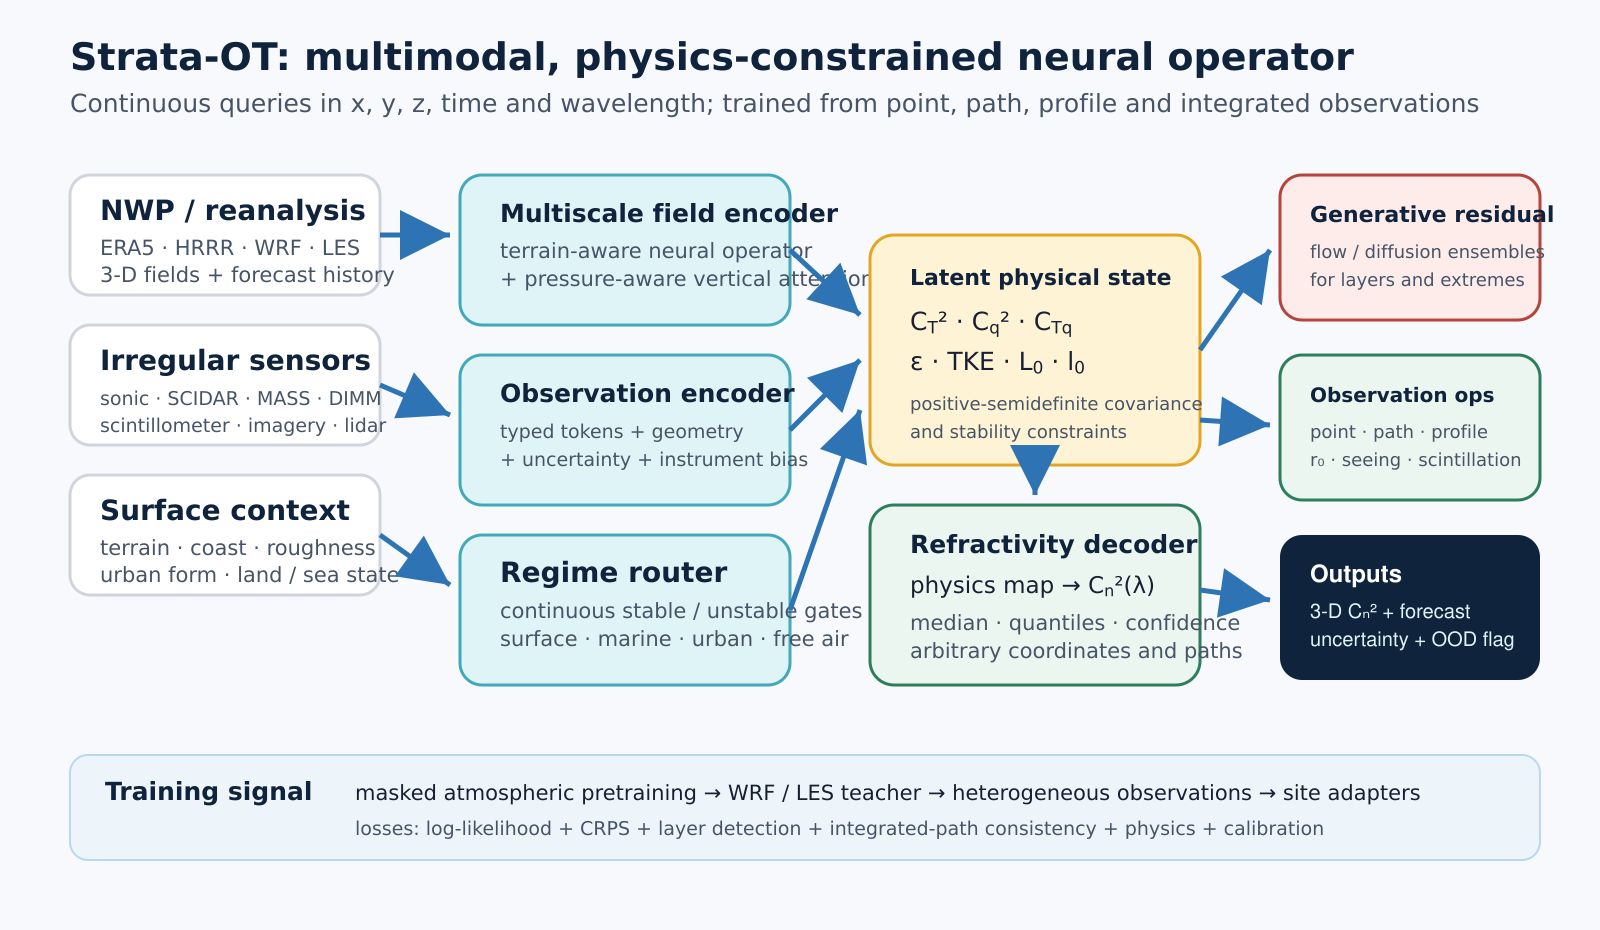
\includegraphics[width=\linewidth]{briefing-assets/media/7ecd842a5a924643d63e8695f6dc84e556b62425.png} \\
\end{longtable}

Prepared \textbf{29 July 2026} · \textbf{Unclassified / public sources
only}

\textbf{Implementation update.} The development workstation is an NVIDIA RTX
5080 with 16 GB VRAM, not the 96 GB workstation assumed in the original
briefing draft. The repository therefore begins with a 2--8M-parameter Surface
model and an 8--15M-parameter Column model, then uses approval-gated rented
48--80 GB GPUs only when measured evidence justifies scaling. The publication
marketing site is deferred; the repository includes only a local research
console for runs, data, gates, and system health.

\textbf{How to read this briefing}

\textbf{Scope.} This is an unclassified, public-source research plan for
predicting and representing atmospheric optical turbulence. It
deliberately stops at atmospheric-effects modeling and does not specify
weapon employment, target vulnerability, engagement envelopes, or system
lethality.

\textbf{Evidence standard.} The report distinguishes verified
high-priority papers and datasets from a broader discovery bibliography.
The appendix contains 193 research, technical, standards and
adjacent-architecture references (167 carried forward from the 2025 IEEE
review and 26 post-review or cross-domain sources). Inclusion in the
index does not mean every item was read in full.

\textbf{Originality caveat.} Strata-OT is a novel proposed synthesis for
research planning---not a representation that global prior art,
patentability, or freedom to operate has been established.

\begin{longtable}[]{@{}
  >{\raggedright\arraybackslash}p{(\columnwidth - 2\tabcolsep) * \real{0.0218}}
  >{\raggedright\arraybackslash}p{(\columnwidth - 2\tabcolsep) * \real{0.9782}}@{}}
\toprule\noalign{}
\endhead
\bottomrule\noalign{}
\endlastfoot
& \textbf{NAMING NOTE}

``Strata-OT'' is a descriptive research codename used throughout. Run
trademark, domain and program-security checks before adopting it
publicly. \\
\end{longtable}

\textbf{Contents}

\begin{itemize}
\item
  1. Executive decision and viability
\item
  2. The modeling problem: what Cn² is and why it is hard
\item
  3. Research landscape and state of the art
\item
  4. Dataset landscape and the OpenCn2 data program
\item
  5. Proposed architecture: Strata-OT
\item
  6. Model family, training strategy and compute
\item
  7. Evaluation protocol and acceptance gates
\item
  8. Research hypotheses and experiment portfolio
\item
  9. Twelve-month execution roadmap
\item
  10. Publication website and product experience
\item
  11. Security, release and dual-use boundaries
\item
  12. Recommendations and 30-day start
\item
  Appendices: dataset cards, experiment backlog, bibliography
\end{itemize}

\textbf{1. Executive decision and viability}

\emph{The core idea is scientifically credible and timely. The limiting
factor is not whether neural networks can learn Cn²; it is whether the
data, observation geometry and evaluation design are strong enough to
support transfer beyond one site.}

\begin{longtable}[]{@{}
  >{\raggedright\arraybackslash}p{(\columnwidth - 2\tabcolsep) * \real{0.0218}}
  >{\raggedright\arraybackslash}p{(\columnwidth - 2\tabcolsep) * \real{0.9782}}@{}}
\toprule\noalign{}
\endhead
\bottomrule\noalign{}
\endlastfoot
& \textbf{RECOMMENDATION: PHASE-GATED GO}

Fund a 12-month research program whose first products are (1) an
expanded OpenCn2 benchmark and common data schema, (2) a
20--120M-parameter profile/nowcast model, and (3) a public research
site. Defer any 300M--1B regional foundation model until cross-site
field results justify scaling. \\
\end{longtable}

\begin{longtable}[]{@{}
  >{\raggedright\arraybackslash}p{(\columnwidth - 4\tabcolsep) * \real{0.2350}}
  >{\raggedright\arraybackslash}p{(\columnwidth - 4\tabcolsep) * \real{0.1816}}
  >{\raggedright\arraybackslash}p{(\columnwidth - 4\tabcolsep) * \real{0.5833}}@{}}
\toprule\noalign{}
\begin{minipage}[b]{\linewidth}\raggedright
\textbf{Dimension}
\end{minipage} & \begin{minipage}[b]{\linewidth}\raggedright
\textbf{Assessment}
\end{minipage} & \begin{minipage}[b]{\linewidth}\raggedright
\textbf{Why}
\end{minipage} \\
\midrule\noalign{}
\endhead
\bottomrule\noalign{}
\endlastfoot
Scientific learnability & HIGH & Direct ML studies already show useful
scalar and profile skill; physics constraints offer a plausible path to
transfer. \\
Public direct-label data & LOW--MEDIUM & Several good datasets exist,
but they are sparse, heterogeneous and concentrated in observatory or
fixed-path regimes. \\
Covariate / pretraining data & HIGH & ERA5, ERA5-Land, HRRR, WRF and
field-campaign turbulence data provide enormous atmospheric context. \\
Novel research headroom & HIGH & No public work combines continuous 3-D
querying, heterogeneous observation operators, latent refractivity
physics and generative extreme-layer residuals. \\
Single-GPU feasibility & HIGH for MVP & An RTX 5080 with 16 GB can train
the compact Surface and first Column models with BF16, bounded context,
and accumulation; larger profile or regional work moves to a rented
48--80 GB GPU only after local evidence gates pass. \\
Universal operational model & MEDIUM--LOW near term & Urban, maritime,
coastal, complex-terrain and free-atmosphere transfer remain unresolved;
direct HEL datasets are often controlled. \\
Publication / product value & HIGH & A benchmark plus transparent
uncertainty and a polished interactive site would be useful across
astronomy, FSO, imaging and defense research. \\
\end{longtable}

\textbf{The investable thesis}

\begin{itemize}
\item
  \textbf{Do not build ``a better ExtraTrees model.''} Build a
  continuous atmospheric operator that can be queried at arbitrary
  altitude, time, wavelength and path geometry.
\item
  \textbf{Do not train only on a single label type.} Use differentiable
  observation operators so point, path-averaged, layered and integrated
  observations can supervise one latent turbulence state.
\item
  \textbf{Do not optimize only mean error.} Explicitly target rare
  strong layers, regime transitions, calibration and out-of-distribution
  detection.
\item
  \textbf{Do not confuse model size with a data moat.} The durable asset
  is the normalized multisite corpus, benchmark protocol and instrument
  metadata.
\item
  \textbf{Do not publish a defense-integrated stack.} Publish an open
  atmospheric core and keep controlled adapters, data and system
  integration on a separate governed path.
\end{itemize}

\textbf{What success would look like}

A successful first-generation system predicts log₁₀(Cn²) profiles and
short-horizon evolution with calibrated uncertainty; transfers to
withheld sites better than climatology, physics baselines and modern
tabular/tree baselines; preserves localized high-turbulence layers; and
correctly identifies when it is outside its validated domain.

\textbf{2. The modeling problem: what Cn² is and why it is hard}

\emph{Cn² is a scale-dependent statistical descriptor of
refractive-index fluctuations, not a directly resolved weather variable.
The model must infer subgrid turbulence from imperfect environmental
fields and heterogeneous optical measurements.}

\textbf{2.1 Physical definition and useful derived quantities}

In the inertial subrange, the refractive-index structure function is
commonly written \textbf{Dₙ(r) = ⟨{[}n(x+r)−n(x){]}²⟩ ≈ Cₙ² r²/³}. Cₙ²
therefore has units of m⁻²/³ and is normally modeled in log space
because it spans orders of magnitude.
\href{https://ntrl.ntis.gov/NTRL/dashboard/searchResults/titleDetail/TT6850464.xhtml}{\textbf{\ul{TATARSKII}}}

A useful physically explicit decomposition is \textbf{Cₙ² = A\_T² C\_T²
+ A\_q² C\_q² + 2 A\_T A\_q C\_Tq}, where the coefficients depend on
wavelength, pressure, temperature and humidity. The covariance term
matters particularly near moist surfaces and coastal environments; it
also supplies a concrete positivity constraint for a neural latent
state.
\href{https://opg.optica.org/abstract.cfm?uri=josaa-5-4-481}{\textbf{\ul{ANDREAS}}}

Common path metrics are integrals or weighted transforms of the profile.
For a plane wave, for example, \textbf{r₀ = {[}0.423 k² ∫ Cₙ²(z)
dz{]}⁻³/⁵}. Seeing, isoplanatic angle, coherence time, Rytov variance
and scintillation respond to different altitude/path weightings. A model
can have a reasonable average profile and still be wrong for the
quantity a downstream propagation model uses.

\begin{longtable}[]{@{}
  >{\raggedright\arraybackslash}p{(\columnwidth - 2\tabcolsep) * \real{0.0218}}
  >{\raggedright\arraybackslash}p{(\columnwidth - 2\tabcolsep) * \real{0.9782}}@{}}
\toprule\noalign{}
\endhead
\bottomrule\noalign{}
\endlastfoot
& \textbf{MODELING IMPLICATION}

Train against both local Cn² and differentiable integrated observables.
A profile-only loss can reward vertically smoothed answers that look
plausible but underestimate thin, strong layers and produce optimistic
propagation metrics. \\
\end{longtable}

\textbf{2.2 Why this is a persistent pain point}

\begin{itemize}
\item
  \textbf{Subgrid physics:} The turbulence scales relevant to optical
  propagation are far smaller than global or mesoscale weather grids.
\item
  \textbf{Boundary-layer nonstationarity:} Surface heating, stability
  transitions, wakes, terrain, coastlines and urban form create sharp
  space-time structure.
\item
  \textbf{Multiple definitions of ``ground truth'':} Sonic estimates are
  local, scintillometers are path weighted, DIMM/MASS/SCIDAR invert
  different optical observables, and NWP products are model-derived.
\item
  \textbf{Instrument bias and geometry:} Height, aperture, wavelength,
  alignment, path weighting and processing choices materially affect
  labels.
\item
  \textbf{Log-heavy tails:} Rare strong turbulence and intermittent
  layers are operationally important but underrepresented in standard
  losses.
\item
  \textbf{Domain shift:} A model can interpolate beautifully at one site
  while failing across seasons, instruments, terrain or a land--sea
  boundary.
\item
  \textbf{Teacher bias:} WRF/LES-generated labels enable scale, but a
  student trained only on a parameterization cannot exceed the teacher's
  physical assumptions without field data.
\end{itemize}

\textbf{2.3 Defense / HEL relevance without overclaiming}

Atmospheric turbulence changes wavefront coherence, beam spread,
scintillation and adaptive-optics burden. Public defense literature
describes the difficulty of representing low-altitude, maritime and
land--sea-interface turbulence in laser-performance models, and public
budgets continue to support directed-energy atmospheric propagation
research. The proposed work should therefore be positioned as an
atmospheric-effects and uncertainty layer that can feed authorized
propagation environments---not as an end-to-end engagement predictor.

\textbf{3. Research landscape and state of the art}

\emph{The literature has moved from static climatologies and similarity
models to NWP-coupled parameterizations, local machine learning, deep
profile reconstruction and foundation-model transfer. The strongest
modern result is not that one architecture has solved the problem; it is
that hybrid physics/data approaches repeatedly generalize better.}

\textbf{3.1 Method families}

\begin{longtable}[]{@{}
  >{\raggedright\arraybackslash}p{(\columnwidth - 6\tabcolsep) * \real{0.1763}}
  >{\raggedright\arraybackslash}p{(\columnwidth - 6\tabcolsep) * \real{0.2618}}
  >{\raggedright\arraybackslash}p{(\columnwidth - 6\tabcolsep) * \real{0.2778}}
  >{\raggedright\arraybackslash}p{(\columnwidth - 6\tabcolsep) * \real{0.2842}}@{}}
\toprule\noalign{}
\begin{minipage}[b]{\linewidth}\raggedright
\textbf{Family}
\end{minipage} & \begin{minipage}[b]{\linewidth}\raggedright
\textbf{Representative methods}
\end{minipage} & \begin{minipage}[b]{\linewidth}\raggedright
\textbf{Strength}
\end{minipage} & \begin{minipage}[b]{\linewidth}\raggedright
\textbf{Failure mode}
\end{minipage} \\
\midrule\noalign{}
\endhead
\bottomrule\noalign{}
\endlastfoot
Static / altitude-only & Hufnagel--Valley, Bufton, Gurvich & Cheap,
stable, easy to integrate & Cannot represent local instantaneous layers
or boundary-layer transitions \\
Empirical macro-meteorology & Sadot, Tunick CN2, coastal regressions &
Uses routine sensors; interpretable & Site-specific coefficients and
limited regimes \\
Similarity / physics & MOST, Tatarskii variants, Andreas marine bulk,
variance based & Physical scaling and better extrapolation & Requires
fluxes/gradients/outer scales that are uncertain or unresolved \\
NWP-coupled & WRF optical turbulence, MOSE/ALTA, Quatresooz hybrid BL/FA
& 3-D time-varying fields and forecasts & Expensive; sensitive to grid,
PBL scheme and parameterization \\
Local classical ML & MLP, GBRT, random forest, Pi-ML, OTCliM & Strong
same-site skill and fast inference & Transfer and tail behavior often
weak; most output a scalar \\
Deep profile / sensing & OTProf, video physics-CNN, neural
scintillometry, OCAN & Profile structure, raw-sensor learning and larger
representation capacity & Data hungry; still narrow domains; smoothing
and synthetic labels \\
Proposed next step & Strata-OT continuous multimodal operator & One
latent state supervised by many observation geometries; probabilistic
extremes & Higher engineering burden; needs disciplined benchmark and
calibration \\
\end{longtable}

\textbf{3.2 What the direct evidence says}

\textbf{OTProf is the closest direct architectural precedent.} Its
Squeezeformer combines convolution and attention, interpolates from 30
to 100 vertical levels in feature space, and predicts Cₙ² together with
turbulence variables. On its ERA5 inference test it reports materially
better profile statistics than Hufnagel--Valley. The critical warning is
equally important: rare strong events are smoothed, which can bias
Fried-parameter and scintillation estimates in an optimistic direction.
\href{https://arxiv.org/abs/2604.09346}{\textbf{\ul{PAPER}}}

\textbf{Few-shot transfer is already plausible.} Basu's 2026 study
applies pretrained tabular foundation models to the Mauna Loa campaign.
Performance rises substantially as the label budget grows from one to
eighteen days, indicating that a pretrained atmospheric backbone plus
small local adapters is a credible design pattern.
\href{https://doi.org/10.1364/AO.585045}{\textbf{\ul{PAPER}}}

\textbf{Purely learned sensing can scale, but domain lock-in is real.}
The 2026 Chesapeake Bay CNN study uses more than twelve million laser
images, while the public video study shows that a naive CNN performs
well inside one scene and transfers poorly. The physics-coupled image
gradient branch materially improves transfer.
\href{https://opg.optica.org/ao/abstract.cfm?uri=ao-65-19-H86}{\textbf{\ul{BASS}}}
\href{https://arxiv.org/abs/2408.16623}{\textbf{\ul{SAHA}}}

\textbf{The benchmarking community has identified the exact research
risk.} otbench emphasizes blocked operational tasks and long-duration
datasets because random train/test rows can create spectacular but
misleading scores. The 2025 review likewise concludes that location- and
season-independent models, easily obtained meteorology, manageable
calibration and separate boundary/free-atmosphere treatment are the
desired direction.
\href{https://arxiv.org/abs/2401.03573}{\textbf{\ul{OTBENCH}}}
\href{https://doi.org/10.1109/ACCESS.2025.3535093}{\textbf{\ul{REVIEW}}}

\begin{longtable}[]{@{}
  >{\raggedright\arraybackslash}p{(\columnwidth - 2\tabcolsep) * \real{0.0218}}
  >{\raggedright\arraybackslash}p{(\columnwidth - 2\tabcolsep) * \real{0.9782}}@{}}
\toprule\noalign{}
\endhead
\bottomrule\noalign{}
\endlastfoot
& \textbf{SYNTHESIS}

The publishable gap is not ``try a Transformer.'' It is to combine
continuous operator learning, heterogeneous measurement physics, latent
thermodynamic covariance, regime routing, calibrated uncertainty and a
residual generator designed specifically to recover intermittent
vertical structure. \\
\end{longtable}

\textbf{3.3 High-priority paper map}

The table below is the compact reading list. It separates evidence that
directly informs Cn² modeling from adjacent architecture evidence used
to justify the proposed design.

\begin{longtable}[]{@{}
  >{\raggedright\arraybackslash}p{(\columnwidth - 6\tabcolsep) * \real{0.1229}}
  >{\raggedright\arraybackslash}p{(\columnwidth - 6\tabcolsep) * \real{0.2831}}
  >{\raggedright\arraybackslash}p{(\columnwidth - 6\tabcolsep) * \real{0.3216}}
  >{\raggedright\arraybackslash}p{(\columnwidth - 6\tabcolsep) * \real{0.2724}}@{}}
\toprule\noalign{}
\begin{minipage}[b]{\linewidth}\raggedright
\textbf{Area}
\end{minipage} & \begin{minipage}[b]{\linewidth}\raggedright
\textbf{Paper / resource}
\end{minipage} & \begin{minipage}[b]{\linewidth}\raggedright
\textbf{What it contributes}
\end{minipage} & \begin{minipage}[b]{\linewidth}\raggedright
\textbf{Important limitation}
\end{minipage} \\
\midrule\noalign{}
\endhead
\bottomrule\noalign{}
\endlastfoot
Review &
\href{https://doi.org/10.1109/ACCESS.2025.3535093}{\textbf{\ul{Cn²
Modeling for Free-Space Optical Communications: A Review}}} & Best
current taxonomy of altitude-only, parametric, boundary-layer, NWP and
ML models; makes multisite validation and hybrid
boundary/free-atmosphere modeling explicit priorities. & FSO framing;
conclusions still transfer strongly to HEL atmospheric-effects
modeling. \\
Deep profile &
\href{https://arxiv.org/abs/2604.09346}{\textbf{\ul{OTProf: estimating
high-resolution profiles of Cn² from reanalysis using deep learning}}} &
A \textasciitilde1M-parameter Squeezeformer maps 30 pressure levels to
100-level profiles and beats Hufnagel--Valley on ERA5-driven tests. &
Targets are WRF-derived; rare strong layers are smoothed and integrated
effects can become optimistic. \\
Foundation model &
\href{https://doi.org/10.1364/AO.585045}{\textbf{\ul{Leveraging deep
learning-based foundation models for Cn² estimation under data
scarcity}}} & Tabular foundation models reach useful few-shot
performance on Mauna Loa and improve materially with days rather than
months of labels. & One surface-layer campaign; foundation prior is
tabular, not atmospheric or profile-native. \\
Physics + ML &
\href{https://doi.org/10.1364/OL.492652}{\textbf{\ul{Pi-ML:
dimensional-analysis-based ML parameterization of surface-layer optical
turbulence}}} & Shows that non-dimensional, physically meaningful
variables can deliver strong accuracy and recover interpretable
scalings. & Gradient-boosted trees and surface-layer scope; useful
baseline, not the requested advanced architecture. \\
Benchmarking &
\href{https://arxiv.org/abs/2401.03573}{\textbf{\ul{Effective Benchmarks
for Optical Turbulence Modeling}}} & Introduces otbench tasks,
operationally meaningful splits, multiple direct Cn² datasets, and
baseline models. & Current task and model coverage is still small; it
should be extended rather than treated as finished. \\
Near-surface &
\href{https://arxiv.org/abs/2408.00520}{\textbf{\ul{OTCliM: generating a
near-surface Cn² climatology using gradient boosting}}} & One year of
labels plus ERA5 extrapolates four held-out years across 17 New York
stations; cross-site transfer is possible outside difficult urban
regimes. & Climatology and tree model; urban generalization remains
weak. \\
Parameterization &
\href{https://opg.optica.org/ao/abstract.cfm?uri=ao-63-16-E107}{\textbf{\ul{Intercomparison
of flux-, gradient-, and variance-based Cn² parameterizations}}} & The
variance-based parameterization is a strong physics teacher and
generally outperforms the alternatives under the study conditions. &
Scintillometer validation labels are not publicly released; two sites
cannot establish universal validity. \\
Neural regression &
\href{https://doi.org/10.1364/AO.532723}{\textbf{\ul{Estimation of
ground-based atmospheric turbulence strength by neural network
architecture}}} & A modern feed-forward neural design beats tree
baselines and retains some out-of-distribution skill. & Data are not
public and outputs are ground-based scalar Cn², not 3-D fields. \\
Video sensing &
\href{https://arxiv.org/abs/2408.16623}{\textbf{\ul{Turbulence Strength
Cn² Estimation from Video using Physics-based Deep Learning}}} & Public
colocated video/scintillometer data; physics-coupled CNN transfers far
better than a pure image regressor. & Only two short Arizona
collections; video is an observation modality, not a weather forecast
solution. \\
Laser sensing &
\href{https://opg.optica.org/ao/abstract.cfm?uri=ao-65-19-H86}{\textbf{\ul{Estimating
atmospheric Cn² using deep convolutional neural networks}}} & Twelve
million pupil-plane images over nearly five months and a 16.2-km
Chesapeake Bay link demonstrate neural scintillometry at meaningful
scale. & The training corpus is not advertised as open; a single link
geometry risks domain lock-in. \\
Profile archive &
\href{https://arxiv.org/abs/2607.25940}{\textbf{\ul{CNN-Based Reanalysis
of Optical Turbulence at the Canary Islands Observatories (OCAN)}}} &
Nearly 300 nights and hundreds of thousands of g-SCIDAR profiles show
the scale available in observatory archives. & Very new preprint;
current work clusters profile heatmaps rather than forecasting them, and
database access is unclear. \\
Classical ANN &
\href{https://doi.org/10.1364/OL.41.002334}{\textbf{\ul{Using an
artificial neural network to estimate surface-layer turbulence at Mauna
Loa}}} & Establishes the learnability of Cn² from temperature, humidity,
pressure, potential-temperature gradient and wind shear. & Single hidden
layer, single site and limited campaign duration. \\
Hybrid local &
\href{https://opg.optica.org/ao/abstract.cfm?uri=ao-62-18-4880}{\textbf{\ul{Hybrid
optical turbulence models using machine learning and local
measurements}}} & Physics/macro-meteorological baselines plus small
local datasets improve rapidly---sometimes after one or two days of
observations. & Gradient-boosted trees and scalar near-surface
observations. \\
Maritime &
\href{https://opg.optica.org/ao/abstract.cfm?uri=ao-60-11-2938}{\textbf{\ul{Machine-learning
informed macro-meteorological models for the near-maritime
environment}}} & Shows the value and difficulty of maritime variables
and long-duration local measurement. & Site dependence and
instrument-specific effects remain substantial. \\
Maritime &
\href{https://opg.optica.org/ao/abstract.cfm?uri=ao-59-21-6379}{\textbf{\ul{Machine
learning informed predictor importance measures in maritime optical
turbulence}}} & Provides defensible predictor-importance evidence for
surface heat exchange, temperature contrast and related
macro-meteorology. & Importance is model- and dataset-dependent; it is
not causal identification. \\
Marine profile &
\href{https://doi.org/10.3390/rs14092267}{\textbf{\ul{Optical turbulence
profile in marine environment with artificial neural network model}}} &
Demonstrates neural profile estimation in a marine regime rather than a
dry astronomical site. & Regional validation and profile-label
provenance limit transfer claims. \\
Mountain profile &
\href{https://doi.org/10.1093/mnras/stab1829}{\textbf{\ul{In situ
measurements and neural network analysis over the Tibetan Plateau}}} &
Connects in-situ vertical profile measurements with neural analysis in
complex high terrain. & Campaign and geography are specialized. \\
NWP & \href{https://doi.org/10.1364/OE.498401}{\textbf{\ul{Continuous
daytime and nighttime forecast from numerical weather prediction
models}}} & Shows that operationally available meteorological forecasts
can support continuous Cn² forecasting with explicit boundary-layer
treatment. & NWP resolution and site calibration remain limiting. \\
NWP &
\href{https://ui.adsabs.harvard.edu/abs/1999A\%26AS..137..185M/abstract}{\textbf{\ul{3D
mapping of optical turbulence using an atmospheric numerical model}}} &
Foundational demonstration that mesoscale models can create time-varying
3-D optical-turbulence fields. & Computationally expensive and dependent
on parameterization choices. \\
NWP &
\href{https://journals.ametsoc.org/view/journals/apme/47/4/2007jamc1524.1.xml}{\textbf{\ul{Modeling
optical turbulence and seeing over Mauna Kea}}} & Links mesoscale
meteorology to observed seeing at a demanding mountain site. &
Astronomical vertical-path use and one geographic regime. \\
Physics &
\href{https://doi.org/10.1007/s10652-022-09880-3}{\textbf{\ul{Revisiting
and revising Tatarskii's formulation for C\_T²}}} & Derives a
variance/flux-budget-based formulation and a physically based outer
scale from routine meteorology. & A parameterization is not a complete
data assimilation or forecasting model. \\
Physics & \href{https://doi.org/10.1364/OL.40.000321}{\textbf{\ul{A
high-order physically based Cn² parameterization}}} & Provides a
free-atmosphere formulation with desirable limiting behavior and
stronger mountain-wave performance than common alternatives. & Still
depends on resolved gradients and turbulence quantities from a host
model. \\
Marine physics &
\href{https://journals.ametsoc.org/view/journals/apme/39/10/1520-0450-39.10.1770.xml}{\textbf{\ul{Estimating
Cn² over the ocean using bulk methods}}} & Canonical treatment of
temperature/humidity covariance and sea-surface exchange for maritime
propagation. & Homogeneous bulk assumptions fail near wakes, coastlines
and sharp land--sea transitions. \\
Surface physics &
\href{https://doi.org/10.1016/S1364-8152(02)00052-X}{\textbf{\ul{CN2
model for micrometeorological influences on refractive-index
structure}}} & Widely used Army-origin semi-empirical land model from
two-level conventional meteorology. & Strong assumptions and local
calibration limit universality. \\
Observation &
\href{https://doi.org/10.1029/2022RS007624}{\textbf{\ul{Computation of
Cn² from its statistical definition using radiosonde data}}} & Offers a
direct statistical route to profile labels from high-resolution
soundings. & Standard radiosonde sampling may miss the scales required
for reliable turbulence retrieval. \\
Generative &
\href{https://opg.optica.org/ao/abstract.cfm?uri=ao-65-13-4525}{\textbf{\ul{Data-driven
learning of atmospheric turbulence phase screens via diffusion models}}}
& Shows diffusion can reproduce complex non-Kolmogorov phase-screen
statistics without GAN instability. & Demonstration data are
simulator-generated; phase screens are downstream of Cn² inference. \\
Forecast uncertainty &
\href{https://arxiv.org/abs/2602.07780}{\textbf{\ul{Short-Term
Turbulence Prediction for Seeing Using Machine Learning}}} &
Normalizing-flow time-series forecasts show how to produce calibrated
distributions rather than only point estimates. & Seeing forecast, not
Cn² field reconstruction. \\
Neural operator &
\href{https://arxiv.org/abs/2010.08895}{\textbf{\ul{Fourier Neural
Operator for Parametric Partial Differential Equations}}} & Supports
grid-independent field-to-field learning and zero-shot super-resolution
in turbulent PDE problems. & Generic PDE benchmark evidence; atmospheric
turbulence needs geometry and sensor-aware extensions. \\
Operator learning &
\href{https://doi.org/10.1038/s42256-021-00302-5}{\textbf{\ul{Learning
nonlinear operators via DeepONet}}} & Provides a principled branch/trunk
formulation for querying continuous output coordinates. & Vanilla
DeepONet is not sufficient for multiscale 3-D atmospheric data. \\
Generative downscale &
\href{https://doi.org/10.1038/s43247-025-02042-5}{\textbf{\ul{Residual
corrective diffusion modeling for km-scale atmospheric downscaling}}} &
Regression-plus-generative residual separates predictable means from
stochastic fine-scale detail---a direct answer to smoothed turbulence
layers. & Weather variables at kilometer scale, not Cn² at
optical-turbulence scales. \\
Weather FM &
\href{https://doi.org/10.1038/s41586-025-09005-y}{\textbf{\ul{A
foundation model for the Earth system (Aurora)}}} & Demonstrates
transfer from a large, heterogeneous atmospheric pretraining corpus to
multiple prediction tasks. & Scale and data budget are far beyond the
direct Cn² corpus. \\
Hybrid weather &
\href{https://doi.org/10.1038/s41586-024-07744-y}{\textbf{\ul{Neural
general circulation models for weather and climate (NeuralGCM)}}} &
Evidence that learned physics and differentiable dynamical structure can
outperform purely black-box or purely numerical components. & Global
circulation scale; use as an architectural principle, not a drop-in
solution. \\
\end{longtable}

\textbf{4. Dataset landscape and the OpenCn2 data program}

\emph{There is enough open material for a serious benchmark and first
model, but not enough direct, standardized Cn² coverage to justify a
universal claim. Data harmonization is therefore a primary research
output.}

\textbf{4.1 Available resources}

\begin{longtable}[]{@{}
  >{\raggedright\arraybackslash}p{(\columnwidth - 10\tabcolsep) * \real{0.0748}}
  >{\raggedright\arraybackslash}p{(\columnwidth - 10\tabcolsep) * \real{0.2083}}
  >{\raggedright\arraybackslash}p{(\columnwidth - 10\tabcolsep) * \real{0.2393}}
  >{\raggedright\arraybackslash}p{(\columnwidth - 10\tabcolsep) * \real{0.1389}}
  >{\raggedright\arraybackslash}p{(\columnwidth - 10\tabcolsep) * \real{0.1752}}
  >{\raggedright\arraybackslash}p{(\columnwidth - 10\tabcolsep) * \real{0.1635}}@{}}
\toprule\noalign{}
\begin{minipage}[b]{\linewidth}\raggedright
\textbf{Tier}
\end{minipage} & \begin{minipage}[b]{\linewidth}\raggedright
\textbf{Resource}
\end{minipage} & \begin{minipage}[b]{\linewidth}\raggedright
\textbf{Labels / scale}
\end{minipage} & \begin{minipage}[b]{\linewidth}\raggedright
\textbf{Access}
\end{minipage} & \begin{minipage}[b]{\linewidth}\raggedright
\textbf{Best use}
\end{minipage} & \begin{minipage}[b]{\linewidth}\raggedright
\textbf{Main risk}
\end{minipage} \\
\midrule\noalign{}
\endhead
\bottomrule\noalign{}
\endlastfoot
A & \href{https://github.com/CDJellen/otbench}{\textbf{\ul{otbench:
MLO\_Cn2 + USNA Cn² tasks}}} & Direct surface / path-averaged Cn² +
meteorology. Multiple benchmark tasks; regression and forecast splits. &
Open code/data loader; MIT package & First reproducible benchmark and
baselines & Few environments; inspect task licenses and missingness \\
A &
\href{https://www.eol.ucar.edu/field_projects/mlocn2}{\textbf{\ul{NCAR
MLO\_CN2}}} & High-rate sonic-derived surface-layer turbulence. 9 Jun--8
Aug 2006, Mauna Loa. & Open NCAR/EOL archive & Few-shot, local transfer
and surface physics & Single high-altitude dry site; short campaign \\
A & \href{https://sitedata.tmt.org/}{\textbf{\ul{TMT Site Testing
Database}}} & MASS/DIMM, SODAR, weather, sonic; profile/integrated
products. Five candidate sites, roughly 2--5 years. & Free with login
and publication conditions & Leave-one-site-out profile and instrument
transfer & Data intentionally unfiltered; rigorous QC required \\
A &
\href{https://archive.eso.org/wdb/help/eso/ambient_paranal.html}{\textbf{\ul{ESO
Paranal Ambient / ASM}}} & DIMM Cn²/seeing, MASS 6-layer profile, SLODAR
surface layer, met. DIMM since 1998; MASS since 2016; SLODAR 2016--2020.
& Open query/download interface & Long temporal holdouts, profile +
integrated multitask learning & Astronomical line-of-sight and nighttime
selection effects \\
A− & \href{https://doi.org/10.5281/zenodo.20733692}{\textbf{\ul{OTProf
WRF--ERA5 corpus}}} & Teacher Cn² profiles + TKE, θ variance and length
scale. 25.7 GB; paired high-/coarse-resolution columns. & Open Zenodo +
code & Pretraining, profile decoder reproduction, architecture baseline
& Synthetic teacher bias; not independent ground truth \\
B+ & \href{https://doi.org/10.5281/zenodo.10966120}{\textbf{\ul{WRF Cn²
parameterization intercomparison}}} & Post-processed WRF and
meteorology; parameterization outputs. Two study sites / cases. & Open
Zenodo + GitHub & Physics teacher and parameterization benchmark &
Scintillometer validation labels withheld \\
B &
\href{https://github.com/Riponcs/TurbulenceDataset}{\textbf{\ul{Turbulence
Strength Dataset (video + scintillometer)}}} & Images synchronized to
path-averaged Cn². Two Arizona sets, \textasciitilde30k images each. &
Public download + code & Observation encoder and multimodal proof of
concept & Only \textasciitilde5.75 hours, fixed scenes and daytime
illumination \\
B &
\href{https://www.eol.ucar.edu/content/sample-rate-isff-data-cases99}{\textbf{\ul{CASES-99
high-rate surface flux data}}} & 20-Hz 3-D sonic winds and fast scalar
variables. Main tower + six stations; stable boundary layer. & Open
NCAR/EOL NetCDF & Derive C\_T² / stability labels and pretrain
turbulence encoders & Derived rather than optical label; sensor/QC
expertise required \\
B &
\href{https://www.eol.ucar.edu/field_projects/materhorn-x}{\textbf{\ul{MATERHORN-X}}}
& Dense mountain meteorology and turbulence observations. Dry, fall,
spring and fog campaigns. & NCAR/EOL archive & Complex-terrain
representation and regime stress tests & Cn² must be derived or paired
with a physics teacher \\
B &
\href{https://www.eol.ucar.edu/field_projects/perdig\%C3\%A3o}{\textbf{\ul{Perdigão
2017}}} & Dense sonic, mast, lidar and energy-balance observations.
Two-ridge complex terrain; Dec 2016--Jun 2017. & NCAR/EOL archive &
Terrain-aware encoders and multiscale turbulence pretraining & No direct
optical label \\
A covariate &
\href{https://cds.climate.copernicus.eu/datasets/reanalysis-era5-pressure-levels}{\textbf{\ul{ERA5
/ ERA5-Land}}} & Global atmospheric covariates, pressure levels and
surface fields. Hourly, multidecadal global coverage. & Open via
Copernicus CDS terms & Foundation pretraining, historical covariates and
climatology & Coarse boundary layer and terrain; not a Cn² label \\
A covariate &
\href{https://registry.opendata.aws/noaa-hrrr-pds/}{\textbf{\ul{NOAA
HRRR}}} & 3-km hourly analyses/forecasts with rich boundary-layer
fields. CONUS archive since 2014. & Open cloud archive &
Higher-resolution U.S. covariates and forecast-time realism & Model
changes and archive volume; no direct Cn² \\
B+ & \href{https://nysmesonet.org/}{\textbf{\ul{New York State
Mesonet}}} & 5-min surface meteorology; flux network at selected
stations. 127 stations; 17 used by OTCliM. & Data request / terms vary
by use & Near-surface cross-site benchmark and urban/rural regimes &
Access and redistribution constraints; Cn² subset provenance \\
A if licensed & \href{https://arxiv.org/abs/2607.25940}{\textbf{\ul{OCAN
g-SCIDAR profile archive}}} & High-resolution vertical Cn² profiles.
Nearly 300 nights; hundreds of thousands of profiles. & Paper public;
database access not established & Potential profile foundation corpus /
external collaboration & Gated or author-mediated; observatory/nighttime
domain \\
A if licensed &
\href{https://opg.optica.org/ao/abstract.cfm?uri=ao-65-19-H86}{\textbf{\ul{Chesapeake
Bay neural scintillometry corpus}}} & Pupil-plane imagery + path Cn² +
air--water temperature difference. \textgreater12 million images, 16.2
km, nearly five months. & Paper open; corpus availability not stated &
Large-scale optical encoder and instrument modeling & Requires
partnership; one maritime path/instrument \\
Teacher only &
\href{https://www2.mmm.ucar.edu/wrf/users/}{\textbf{\ul{On-demand WRF /
LES / phase-screen generation}}} & Synthetic latent physics, Cn²
teachers and optical observables. Controllable, effectively unlimited. &
Open software; compute- and expertise-intensive & Coverage of rare
regimes, pretraining and controlled ablations & Simulation bias must
never be confused with field truth \\
\end{longtable}

\textbf{4.2 Data taxonomy: never merge unlike labels blindly}

\begin{longtable}[]{@{}
  >{\raggedright\arraybackslash}p{(\columnwidth - 6\tabcolsep) * \real{0.1389}}
  >{\raggedright\arraybackslash}p{(\columnwidth - 6\tabcolsep) * \real{0.1923}}
  >{\raggedright\arraybackslash}p{(\columnwidth - 6\tabcolsep) * \real{0.2949}}
  >{\raggedright\arraybackslash}p{(\columnwidth - 6\tabcolsep) * \real{0.3739}}@{}}
\toprule\noalign{}
\begin{minipage}[b]{\linewidth}\raggedright
\textbf{Label class}
\end{minipage} & \begin{minipage}[b]{\linewidth}\raggedright
\textbf{Examples}
\end{minipage} & \begin{minipage}[b]{\linewidth}\raggedright
\textbf{What the model actually observes}
\end{minipage} & \begin{minipage}[b]{\linewidth}\raggedright
\textbf{Required metadata}
\end{minipage} \\
\midrule\noalign{}
\endhead
\bottomrule\noalign{}
\endlastfoot
Point / local & Sonic-derived C\_T²/Cn², tower estimates & Turbulence
around an instrument volume and averaging window & Height, sampling
rate, structure-function/spectral method, QC \\
Path weighted & Large-aperture scintillometer, laser link & Integral
with instrument-specific spatial weighting & Endpoints, path height,
wavelength, aperture, weighting kernel, alignment \\
Layered / profile & MASS, SCIDAR, SLODAR, thermosonde & Inverted layer
strengths or high-resolution vertical profile & Vertical response
matrix, altitude coordinates, zenith/airmass, inversion settings \\
Integrated optical & Seeing, r₀, θ₀, τ₀, scintillation & A nonlinear or
weighted functional of Cn² and often wind & Wavelength, geometry,
integration convention, instrument \\
Teacher / synthetic & WRF parameterization, LES, phase-screen simulator
& A model's latent assumptions, not independent truth & Model version,
grid, PBL scheme, parameterization, seed, configuration \\
Proxy & Video distortion, wavefront images, NWP turbulence & A sensor or
host-model signal correlated with turbulence & Full sensor geometry,
exposure, optics, processing and calibration \\
\end{longtable}

\textbf{4.3 Proposed OpenCn2 common schema}

Store a canonical event/observation record plus gridded context. Use
CF-compliant NetCDF/Zarr for atmospheric arrays, Parquet for indexed
observations, and a catalog layer (for example STAC-like assets) for
discoverability. Every label must carry a forward observation operator
or enough metadata to construct one.

\begin{longtable}[]{@{}
  >{\raggedright\arraybackslash}p{(\columnwidth - 2\tabcolsep) * \real{0.2030}}
  >{\raggedright\arraybackslash}p{(\columnwidth - 2\tabcolsep) * \real{0.7970}}@{}}
\toprule\noalign{}
\begin{minipage}[b]{\linewidth}\raggedright
\textbf{Group}
\end{minipage} & \begin{minipage}[b]{\linewidth}\raggedright
\textbf{Minimum fields}
\end{minipage} \\
\midrule\noalign{}
\endhead
\bottomrule\noalign{}
\endlastfoot
Identity / provenance & sample\_id, source\_id, campaign, license,
citation, original checksum, processing version \\
Space-time & UTC start/end, latitude/longitude/altitude, vertical
coordinate type, forecast initialization/lead \\
Geometry & point, path endpoints, ray/zenith geometry, layer response,
footprint and averaging window \\
Instrument & instrument family/model, wavelength, aperture, sampling,
firmware/processing, calibration ID \\
Target & label name, value/log value, units, uncertainty, quality flag,
censoring/saturation \\
Meteorology & T, θ, q/RH, p, u/v/w, radiation, sensible/latent flux,
TKE/PBLH, precipitation/cloud \\
Surface/static & elevation, slope/aspect, roughness, land cover, urban
morphology, soil/sea temperature, coastline distance \\
Split controls & site, campaign, instrument, season, regime, event group
and leakage guard \\
\end{longtable}

\textbf{4.4 Quality control and leakage prevention}

\begin{itemize}
\item
  Preserve raw data; make every cleaned value reproducible from
  versioned transforms.
\item
  Time-align instruments using acquisition clocks and document
  resampling; do not forward-fill across regime transitions.
\item
  Keep measurement uncertainty and instrument identifiers; learn
  optional bias embeddings rather than pretending all devices are
  equivalent.
\item
  Split by contiguous time blocks, campaign and site before creating
  rolling windows or normalization statistics.
\item
  Fit scalers and quantile mappings on training folds only.
\item
  Group colocated or overlapping paths so nearly identical atmosphere
  cannot land in both train and test.
\item
  Flag precipitation, cloud, low signal, saturation, bad alignment and
  invalid turbulence ranges without automatically deleting them.
\item
  Retain extreme events and report coverage; do not let a convenient QC
  rule erase the tails the model must learn.
\end{itemize}

\begin{longtable}[]{@{}
  >{\raggedright\arraybackslash}p{(\columnwidth - 2\tabcolsep) * \real{0.0218}}
  >{\raggedright\arraybackslash}p{(\columnwidth - 2\tabcolsep) * \real{0.9782}}@{}}
\toprule\noalign{}
\endhead
\bottomrule\noalign{}
\endlastfoot
& \textbf{DATA MOAT}

The highest-value deliverable may be a legally redistributable,
geometry-aware benchmark spanning point, path and profile labels with
fixed leave-site and leave-instrument splits. That asset would make
every later architecture experiment faster and more credible. \\
\end{longtable}

\textbf{5. Proposed architecture: Strata-OT}

\emph{Strata-OT is a proposed continuous, physics-constrained,
multimodal neural operator. It predicts a latent turbulence state,
converts it to wavelength-aware Cn² through a differentiable
refractivity layer, and learns from heterogeneous instruments through
observation operators.}

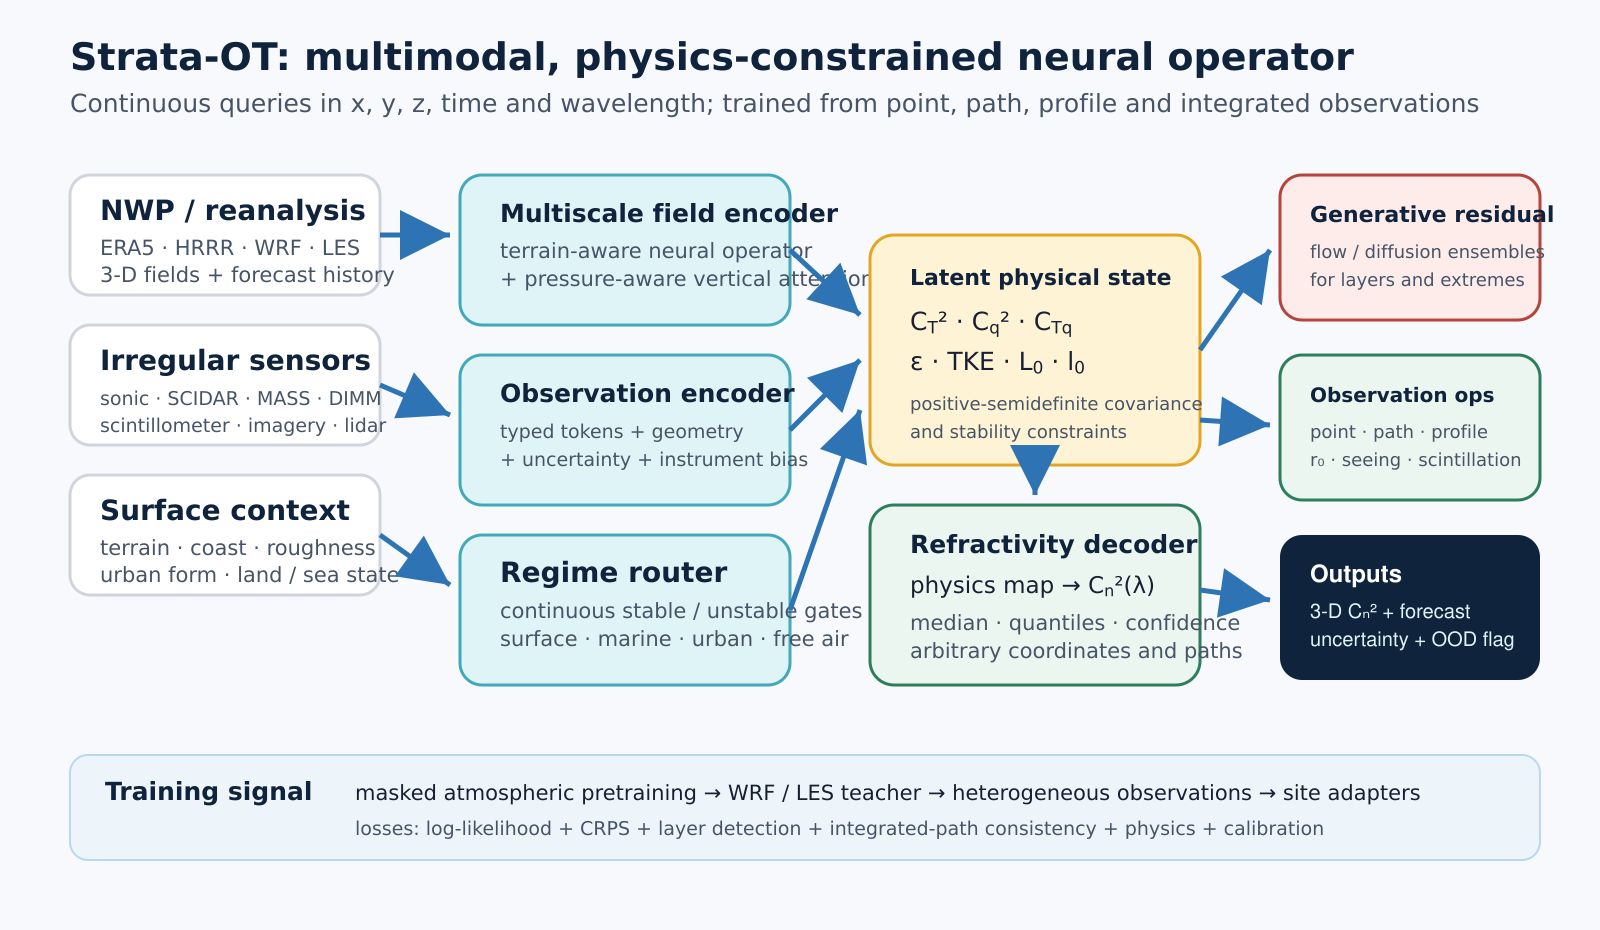
\includegraphics[width=\linewidth]{briefing-assets/media/7ecd842a5a924643d63e8695f6dc84e556b62425.png}

\textbf{Figure 1.} Proposed Strata-OT architecture. This is a research
design, not a reported result.

\textbf{5.1 Continuous query formulation}

Learn an operator \textbf{F: \{atmospheric fields, surfaces,
observations\} → p(s \textbar{} x,y,z,t,λ)}, where s is a latent
turbulence state and the output is a calibrated distribution. A
coordinate-query decoder then returns Cₙ² at arbitrary spatial
coordinates, time, lead and wavelength, rather than at one hard-coded
grid.

This DeepONet-like branch/query separation makes the model usable for
vertical columns, horizontal paths, slant paths and adaptive refinement
without retraining a new output head for every sampling grid. The field
encoder supplies global/regional context; a pressure/height-aware
vertical transformer supplies sharp stratified structure.

\textbf{5.2 Four encoders and a continuous regime router}

\begin{longtable}[]{@{}
  >{\raggedright\arraybackslash}p{(\columnwidth - 6\tabcolsep) * \real{0.1656}}
  >{\raggedright\arraybackslash}p{(\columnwidth - 6\tabcolsep) * \real{0.2083}}
  >{\raggedright\arraybackslash}p{(\columnwidth - 6\tabcolsep) * \real{0.3526}}
  >{\raggedright\arraybackslash}p{(\columnwidth - 6\tabcolsep) * \real{0.2735}}@{}}
\toprule\noalign{}
\begin{minipage}[b]{\linewidth}\raggedright
\textbf{Module}
\end{minipage} & \begin{minipage}[b]{\linewidth}\raggedright
\textbf{Inputs}
\end{minipage} & \begin{minipage}[b]{\linewidth}\raggedright
\textbf{Design}
\end{minipage} & \begin{minipage}[b]{\linewidth}\raggedright
\textbf{Reason}
\end{minipage} \\
\midrule\noalign{}
\endhead
\bottomrule\noalign{}
\endlastfoot
Multiscale field encoder & NWP volumes and history & AFNO/FNO-like
spectral blocks or hierarchical 3-D attention with terrain-aware local
graph edges & Capture synoptic forcing and mesoscale spatial coupling
efficiently \\
Vertical column encoder & Pressure/height levels & Relative pressure,
geopotential and terrain embeddings; axial attention plus local
convolutions & Handle irregular vertical spacing and thin turbulence
layers \\
Observation encoder & Typed sensor tokens & Perceiver/set attention over
location, time, instrument, geometry, uncertainty and measured value &
Assimilate variable numbers and kinds of observations \\
Surface encoder & DEM, roughness, land/sea, urban, radiation &
Multiresolution raster/graph features with solar geometry & Represent
the boundary conditions that dominate near-ground Cn² \\
Regime router & Latent stability and context & Soft mixture-of-experts
gates for stable/neutral/convective, marine/land/urban/terrain and
boundary/free atmosphere & Specialize without brittle hard
classifications or separate disconnected models \\
\end{longtable}

\textbf{5.3 Physics latent state}

Instead of regressing Cₙ² directly from every modality, predict C\_T²,
C\_q² and C\_Tq together with turbulence kinetic energy or dissipation,
an outer/master length scale and optional inner scale. Parameterize the
2×2 temperature--humidity covariance with a Cholesky factor so C\_T² ≥
0, C\_q² ≥ 0 and \textbar C\_Tq\textbar{} ≤ √(C\_T²C\_q²) by
construction.

\begin{itemize}
\item
  A differentiable refractivity layer converts the thermodynamic
  structure parameters to wavelength-aware Cₙ².
\item
  Auxiliary heads for TKE, θ variance and length scale can learn from
  WRF/LES even when direct Cₙ² is absent.
\item
  A physics baseline (variance-based, MOST or free-atmosphere
  parameterization) enters as an explicit residual reference, not as
  unquestioned truth.
\item
  The router can blend surface-layer and free-atmosphere experts
  continuously across the boundary-layer top.
\end{itemize}

\textbf{5.4 Extreme-aware probabilistic residual}

A deterministic profile head predicts the conditional median and
quantiles in log space. A conditional flow-matching or diffusion
residual head learns the unresolved distribution around that mean. This
mirrors successful atmospheric downscaling: regression captures
predictable large-scale structure; the generative residual restores
stochastic layers and calibrated extremes.

\begin{itemize}
\item
  Train the residual on normalized profile innovations and vertical
  gradients, not raw fields, so capacity targets fine structure.
\item
  Use event-balanced sampling and tail-weighted CRPS/quantile losses for
  top-decile and top-percentile layer strength.
\item
  Generate ensembles whose integrated metrics are calibrated; reject
  ``sharp-looking'' profiles that have the wrong r₀ or scintillation
  distribution.
\end{itemize}

\textbf{5.5 Differentiable observation operators}

Each batch may contain a different label type. The latent Cₙ² field is
passed through the appropriate forward operator before comparison with
the observation:

\begin{itemize}
\item
  \textbf{Point operator:} sample the local profile at sensor height and
  averaging window.
\item
  \textbf{Path operator:} integrate with the scintillometer or
  laser-link weighting kernel along the actual geometry.
\item
  \textbf{Layer operator:} apply MASS/SCIDAR/SLODAR vertical response or
  inversion matrix.
\item
  \textbf{Integrated optics:} compute r₀, seeing, θ₀, τ₀ or
  Rytov/scintillation proxies with the documented convention.
\item
  \textbf{Image/wavefront operator:} use a sensor encoder or
  differentiable propagation surrogate only where calibration data
  support it.
\end{itemize}

\textbf{5.6 Objective function}

A practical masked multitask objective is \textbf{L = w\_d L\_direct +
w\_o L\_observation + w\_g L\_gradient + w\_p L\_physics + w\_c
L\_calibration + w\_t L\_tail}. L\_direct is a heteroscedastic log-Cn²
likelihood; L\_observation covers path/layer/integrated metrics;
L\_gradient preserves vertical structure; L\_physics enforces
covariance, stability and baseline consistency; L\_calibration uses
CRPS/coverage; L\_tail protects extremes.

\begin{longtable}[]{@{}
  >{\raggedright\arraybackslash}p{(\columnwidth - 2\tabcolsep) * \real{0.0218}}
  >{\raggedright\arraybackslash}p{(\columnwidth - 2\tabcolsep) * \real{0.9782}}@{}}
\toprule\noalign{}
\endhead
\bottomrule\noalign{}
\endlastfoot
& \textbf{WHY THIS IS MORE THAN A TRANSFORMER}

The novelty is the coupling: continuous coordinate queries +
thermodynamic covariance state + typed observation operators + soft
physical regimes + generative residual ensembles. Any one part exists
elsewhere; their combination is specifically tailored to the Cn² data
problem. \\
\end{longtable}

\textbf{6. Model family, training strategy and compute}

\emph{Build a family around one shared atmospheric representation. The
smaller models validate the science and create deployable artifacts; the
larger model should be earned by data and benchmark gains.}

\textbf{6.1 Proposed family}

\begin{longtable}[]{@{}
  >{\raggedright\arraybackslash}p{(\columnwidth - 8\tabcolsep) * \real{0.1763}}
  >{\raggedright\arraybackslash}p{(\columnwidth - 8\tabcolsep) * \real{0.1335}}
  >{\raggedright\arraybackslash}p{(\columnwidth - 8\tabcolsep) * \real{0.2297}}
  >{\raggedright\arraybackslash}p{(\columnwidth - 8\tabcolsep) * \real{0.2671}}
  >{\raggedright\arraybackslash}p{(\columnwidth - 8\tabcolsep) * \real{0.1934}}@{}}
\toprule\noalign{}
\begin{minipage}[b]{\linewidth}\raggedright
\textbf{Model}
\end{minipage} & \begin{minipage}[b]{\linewidth}\raggedright
\textbf{Approx. size}
\end{minipage} & \begin{minipage}[b]{\linewidth}\raggedright
\textbf{Primary output}
\end{minipage} & \begin{minipage}[b]{\linewidth}\raggedright
\textbf{Inputs}
\end{minipage} & \begin{minipage}[b]{\linewidth}\raggedright
\textbf{Use}
\end{minipage} \\
\midrule\noalign{}
\endhead
\bottomrule\noalign{}
\endlastfoot
Strata-OT Lite & 15--30M & Surface / path Cn², 0--2 h & Local met +
recent labels + optional NWP & Edge/site calibration; fast benchmark
iteration \\
Strata-OT Column & 60--120M & 100--256 level profile, 0--24 h & One NWP
column + surface + optional sensors & First flagship paper and public
API \\
Strata-OT Assimilate & 100--300M & Nowcast profile/field with posterior
uncertainty & Column/field + arbitrary observation tokens & Field
campaigns and instrument fusion \\
Strata-OT Regional & 300--800M & 3-D regional field and ensembles & NWP
tiles/history + terrain + sensors & Regional atmospheric-effects
layer \\
Strata-OT Phase & 150--500M & Conditional phase-screen /
optical-observable ensembles & Predicted Cn², winds, scales and geometry
& Separate research model for propagation simulation \\
Strata-OT Foundation & 1B+ only after gates & Reusable atmospheric
turbulence representation & Multireanalysis + field campaigns +
controlled data & Long-term program, not MVP \\
\end{longtable}

\textbf{6.2 Training curriculum}

\begin{enumerate}
\def\labelenumi{\arabic{enumi}.}
\item
  \textbf{Atmospheric self-supervision.} Masked-variable, masked-level
  and temporal reconstruction on ERA5/ERA5-Land/HRRR; predict gradients,
  stability and flux-related diagnostics.
\item
  \textbf{Physics-teacher pretraining.} Train latent turbulence heads on
  WRF/LES and the OTProf corpus, with teacher/source tokens so the
  network can learn and later correct model-specific bias.
\item
  \textbf{Heterogeneous observation training.} Mix direct datasets using
  masked observation-operator losses and instrument embeddings; use
  balanced sampling by site, regime and label class.
\item
  \textbf{Site adaptation.} Fit low-rank adapters, small calibration
  heads or a neural-process context set from one to several days of
  local observations.
\item
  \textbf{Probabilistic residual.} Freeze or slowly update the
  deterministic backbone while training flow/diffusion innovations and
  calibration.
\item
  \textbf{Continual validation.} Add campaigns only after frozen
  benchmark evaluation; maintain a no-touch external test set and model
  registry.
\end{enumerate}

\textbf{6.3 Compute on an RTX 5080 16 GB, then rented GPUs}

The local GPU is sufficient for meaningful, carefully bounded research.
Start with a 2--8M mixed-precision Surface model and an 8--15M Column
model using BF16, bounded batches, gradient accumulation, and measured
peak VRAM. A validated 60--120M profile model can move to one rented
48--80 GB GPU. Regional and generative experiments remain later,
approval-gated work; throughput and data preprocessing---not only
memory---will become the constraint.

\begin{longtable}[]{@{}
  >{\raggedright\arraybackslash}p{(\columnwidth - 4\tabcolsep) * \real{0.2030}}
  >{\raggedright\arraybackslash}p{(\columnwidth - 4\tabcolsep) * \real{0.3632}}
  >{\raggedright\arraybackslash}p{(\columnwidth - 4\tabcolsep) * \real{0.4338}}@{}}
\toprule\noalign{}
\begin{minipage}[b]{\linewidth}\raggedright
\textbf{Stage}
\end{minipage} & \begin{minipage}[b]{\linewidth}\raggedright
\textbf{Practical compute envelope}
\end{minipage} & \begin{minipage}[b]{\linewidth}\raggedright
\textbf{Expected bottleneck}
\end{minipage} \\
\midrule\noalign{}
\endhead
\bottomrule\noalign{}
\endlastfoot
Baseline reproduction & Hours on the local GPU/CPU node & Data loaders,
exact splits and metrics \\
Surface 2--8M ablations & Bounded runs under four shared GPU-hours &
Campaign mixing, context length and validation \\
Column 8--15M prototype & Hours to a few days locally after Phase 1 &
Profile I/O, vertical resolution and direct-label scarcity \\
Profile 60--120M scale-up & One approved rented 48--80 GB GPU & Live
hourly cost, checkpoint recovery and data placement \\
Regional / generative ensembles & Deferred until profile gates pass &
Spatial tiles, ensemble sampling and evaluation volume \\
1B+ foundation model & Not recommended as the initial goal & Data
diversity, throughput and experimental opportunity cost \\
\end{longtable}

\begin{longtable}[]{@{}
  >{\raggedright\arraybackslash}p{(\columnwidth - 2\tabcolsep) * \real{0.0218}}
  >{\raggedright\arraybackslash}p{(\columnwidth - 2\tabcolsep) * \real{0.9782}}@{}}
\toprule\noalign{}
\endhead
\bottomrule\noalign{}
\endlastfoot
& \textbf{SCALING RULE}

Increase parameter count only when the current model is simultaneously
data-limited less often, underfitting training regimes, and still
improving leave-site performance. Same-site loss alone is not a reason
to scale. \\
\end{longtable}

\textbf{7. Evaluation protocol and acceptance gates}

\emph{A credible result must survive time, site, instrument and regime
shifts. Random row splits should be treated as a debugging check, never
as the headline score.}

\textbf{7.1 Mandatory baselines}

\begin{longtable}[]{@{}
  >{\raggedright\arraybackslash}p{(\columnwidth - 2\tabcolsep) * \real{0.1709}}
  >{\raggedright\arraybackslash}p{(\columnwidth - 2\tabcolsep) * \real{0.8291}}@{}}
\toprule\noalign{}
\begin{minipage}[b]{\linewidth}\raggedright
\textbf{Class}
\end{minipage} & \begin{minipage}[b]{\linewidth}\raggedright
\textbf{Baselines}
\end{minipage} \\
\midrule\noalign{}
\endhead
\bottomrule\noalign{}
\endlastfoot
No-skill & Persistence, diurnal/seasonal climatology, median profile \\
Classical optical & Hufnagel--Valley / site climatology, Tunick CN2,
MOST / Andreas maritime, Trinquet--Vernin or variance-based profile \\
Numerical & Raw WRF/ERA5-derived teacher and any host-model
parameterization \\
Tabular & Linear/elastic net, ExtraTrees, LightGBM/XGBoost, Pi-ML-style
dimensional features, TabPFN/TabDPT where applicable \\
Neural & MLP, TCN/LSTM, 1-D U-Net, Squeezeformer/OTProf reproduction \\
Ablations & No physics state, no observation operators, no regime
router, no residual generator, no pretraining, no instrument
embeddings \\
\end{longtable}

\textbf{7.2 Splits}

\begin{itemize}
\item
  \textbf{Blocked time:} train/validation/test are contiguous and
  normalization is training-only.
\item
  \textbf{Leave site out:} entire geography withheld; report per-site
  and aggregate distributions.
\item
  \textbf{Leave campaign/instrument out:} separate atmospheric transfer
  from instrument calibration memorization.
\item
  \textbf{Regime holdouts:} stable nights, convective afternoons,
  sunrise/sunset transitions, precipitation/cloud, coastal wind sectors,
  strong-shear layers.
\item
  \textbf{Rare-event set:} fixed high-Cn² and thin-layer test slices
  untouched by class balancing.
\item
  \textbf{Forecast realism:} use only data available at initialization
  and distinguish analyses from true forecasts.
\end{itemize}

\textbf{7.3 Metrics: report a panel, not one R²}

\begin{longtable}[]{@{}
  >{\raggedright\arraybackslash}p{(\columnwidth - 2\tabcolsep) * \real{0.2137}}
  >{\raggedright\arraybackslash}p{(\columnwidth - 2\tabcolsep) * \real{0.7863}}@{}}
\toprule\noalign{}
\begin{minipage}[b]{\linewidth}\raggedright
\textbf{Goal}
\end{minipage} & \begin{minipage}[b]{\linewidth}\raggedright
\textbf{Metrics}
\end{minipage} \\
\midrule\noalign{}
\endhead
\bottomrule\noalign{}
\endlastfoot
Point/profile accuracy & MAE and RMSE of log₁₀(Cn²), bias, centered
RMSE, correlation and R² by altitude/regime \\
Vertical structure & Layer location error, layer-strength error,
gradient/spectral distance, integrated error in fixed altitude bands \\
Operational functionals & Relative errors/distributions for r₀, seeing,
θ₀, τ₀ and scintillation/Rytov proxies appropriate to geometry \\
Probabilistic skill & CRPS, NLL, reliability diagram, 50/80/95\%
coverage, interval width and rank histogram \\
Extreme skill & Top-decile/top-percentile recall, precision, quantile
loss and event-conditioned bias \\
Transfer / robustness & Per-site worst case, median improvement,
calibration under shift and OOD AUROC / abstention utility \\
Efficiency & Latency, throughput, memory, ensemble cost and energy for
fixed workloads \\
\end{longtable}

\textbf{7.4 Acceptance gates}

\begin{longtable}[]{@{}
  >{\raggedright\arraybackslash}p{(\columnwidth - 2\tabcolsep) * \real{0.1923}}
  >{\raggedright\arraybackslash}p{(\columnwidth - 2\tabcolsep) * \real{0.8077}}@{}}
\toprule\noalign{}
\begin{minipage}[b]{\linewidth}\raggedright
\textbf{Gate}
\end{minipage} & \begin{minipage}[b]{\linewidth}\raggedright
\textbf{Minimum evidence to proceed}
\end{minipage} \\
\midrule\noalign{}
\endhead
\bottomrule\noalign{}
\endlastfoot
G0 --- Data & Reproduce otbench baselines and at least one published
direct result within documented tolerance; all splits and provenance
frozen. \\
G1 --- Column MVP & Beat the best non-neural baseline on blocked time at
≥3 datasets with calibrated uncertainty and no material tail
regression. \\
G2 --- Transfer & Improve the median leave-site score and avoid
catastrophic degradation on any major environment; report failures
openly. \\
G3 --- Heterogeneous labels & Joint point/path/profile training improves
or preserves each label class versus separate models;
observation-operator ablation is positive. \\
G4 --- Extreme layers & Generative residual improves tail CRPS/layer
recall and integrated metrics without degrading median calibration. \\
G5 --- Scale & Regional model shows meaningful spatial-transfer gains
over independent columns after controlling compute and data. \\
G6 --- Public release & External replication, model/data cards, license
review, security/prepublication review where applicable, and
reproducible artifact hashes. \\
\end{longtable}

\textbf{8. Research hypotheses and experiment portfolio}

\emph{The program should be organized around falsifiable hypotheses.
Architecture components that do not improve transfer, calibration or
tail fidelity should be removed.}

\begin{longtable}[]{@{}
  >{\raggedright\arraybackslash}p{(\columnwidth - 4\tabcolsep) * \real{0.2831}}
  >{\raggedright\arraybackslash}p{(\columnwidth - 4\tabcolsep) * \real{0.4263}}
  >{\raggedright\arraybackslash}p{(\columnwidth - 4\tabcolsep) * \real{0.2906}}@{}}
\toprule\noalign{}
\begin{minipage}[b]{\linewidth}\raggedright
\textbf{Hypothesis}
\end{minipage} & \begin{minipage}[b]{\linewidth}\raggedright
\textbf{Experiment}
\end{minipage} & \begin{minipage}[b]{\linewidth}\raggedright
\textbf{Win condition}
\end{minipage} \\
\midrule\noalign{}
\endhead
\bottomrule\noalign{}
\endlastfoot
H1: latent thermodynamic structure improves transfer & Direct log-Cn²
head vs C\_T²/C\_q²/C\_Tq physics decoder; same parameters and data &
Lower leave-site error and fewer maritime/transition failures \\
H2: observation operators unlock heterogeneous data & Separate models vs
shared latent model with point/path/layer operators & Joint model
improves weighted aggregate without negative transfer \\
H3: residual generation restores thin layers & Quantile-only vs
flow/diffusion residual on OTProf + real profiles & Better tail CRPS,
layer F1 and integrated optics calibration \\
H4: atmospheric pretraining reduces label demand & Random initialization
vs masked ERA5/HRRR pretraining at 1, 3, 7, 30 label days & Higher
few-shot skill and lower cross-site variance \\
H5: soft regime routing beats one monolith & Shared backbone
with/without continuous stability/environment experts & Better
stable/convective and marine/urban worst-case scores \\
H6: sensor context beats fixed calibration & Global instrument
embeddings vs neural-process context set vs per-site fine-tune & Fast
adaptation with fewer labels and honest uncertainty \\
H7: continuous queries improve vertical fidelity & Fixed 100-level
decoder vs coordinate operator at train/test resolutions & Equal or
better error plus reliable super-resolution \\
H8: physics fallback improves safe deployment & OOD detector + physics
fallback vs unconditional neural output & Lower selective risk as
abstention increases \\
\end{longtable}

\textbf{8.1 Publication sequence}

\begin{enumerate}
\def\labelenumi{\arabic{enumi}.}
\item
  \textbf{Paper 1 --- OpenCn2 Benchmark.} Common schema, leakage-safe
  tasks, instrument metadata, classical and neural baselines.
\item
  \textbf{Paper 2 --- Strata-OT Column.} Physics latent state,
  continuous decoder, uncertainty and leave-site results.
\item
  \textbf{Paper 3 --- Heterogeneous Observation Learning.}
  Point/path/profile supervision and few-shot site adaptation.
\item
  \textbf{Paper 4 --- Extreme-Layer Generative Residuals.} Calibrated
  ensembles and downstream optical-integral validation.
\item
  \textbf{Paper 5 --- Regional Neural Operator.} Terrain-aware field
  prediction and independent field-campaign validation.
\end{enumerate}

\textbf{8.2 What would invalidate the thesis}

\begin{itemize}
\item
  Leave-site performance cannot beat simple physics + small local
  calibration even after pretraining.
\item
  Direct datasets disagree so strongly after metadata normalization that
  a shared latent state produces persistent negative transfer.
\item
  Generative residuals improve visual sharpness but not calibrated layer
  or integrated-optics metrics.
\item
  Performance gains disappear when time leakage, teacher overlap and
  instrument identity are controlled.
\item
  Operationally relevant direct data cannot be obtained or released
  under a viable governance model.
\end{itemize}

\begin{longtable}[]{@{}
  >{\raggedright\arraybackslash}p{(\columnwidth - 2\tabcolsep) * \real{0.0218}}
  >{\raggedright\arraybackslash}p{(\columnwidth - 2\tabcolsep) * \real{0.9782}}@{}}
\toprule\noalign{}
\endhead
\bottomrule\noalign{}
\endlastfoot
& \textbf{RESEARCH DISCIPLINE}

A negative result on a universal model can still produce a strong paper
and product: a benchmark that quantifies exactly where local adapters or
physics fallbacks are necessary. \\
\end{longtable}

\textbf{9. Twelve-month execution roadmap}

\emph{The schedule prioritizes reproducibility and direct labels before
model scale. Each phase ends with a concrete artifact and a stop/go
decision.}

\begin{longtable}[]{@{}
  >{\raggedright\arraybackslash}p{(\columnwidth - 6\tabcolsep) * \real{0.1282}}
  >{\raggedright\arraybackslash}p{(\columnwidth - 6\tabcolsep) * \real{0.3205}}
  >{\raggedright\arraybackslash}p{(\columnwidth - 6\tabcolsep) * \real{0.3259}}
  >{\raggedright\arraybackslash}p{(\columnwidth - 6\tabcolsep) * \real{0.2254}}@{}}
\toprule\noalign{}
\begin{minipage}[b]{\linewidth}\raggedright
\textbf{Window}
\end{minipage} & \begin{minipage}[b]{\linewidth}\raggedright
\textbf{Work}
\end{minipage} & \begin{minipage}[b]{\linewidth}\raggedright
\textbf{Deliverables}
\end{minipage} & \begin{minipage}[b]{\linewidth}\raggedright
\textbf{Exit criterion}
\end{minipage} \\
\midrule\noalign{}
\endhead
\bottomrule\noalign{}
\endlastfoot
Weeks 0--4 & Acquire MLO/USNA/TMT/ESO/OTProf; build common schema;
reproduce otbench & Data catalog, checksums, QC notebook, frozen splits,
baseline report & G0 data gate \\
Weeks 5--8 & Implement physics parameterizations and neural baselines;
create evaluation harness & Benchmark dashboard, model registry, metric
suite & Published baselines reproduced \\
Weeks 9--12 & Train Strata-OT Lite/Column v0; uncertainty and coordinate
decoder & v0 weights, ablations, error atlas & Beat baselines on blocked
time \\
Months 4--5 & Atmospheric pretraining and few-shot adapters; add TMT/ESO
profiles & v1 column model, leave-site study, Paper 1 draft & G1/G2
evidence \\
Months 6--7 & Observation-token fusion and path/layer operators &
Assimilate prototype, instrument cards, Paper 2 draft & G3 evidence \\
Months 8--9 & Flow/diffusion residual, extreme-event evaluation &
Calibrated ensembles, tail benchmark, Paper 3/4 draft & G4 evidence \\
Months 10--11 & Regional tiles, terrain graph, public demo APIs &
Regional alpha, inference service, public model/data cards & G5 evidence
or defer scale \\
Month 12 & External replication, release review, polished website &
DOI/archive, documentation, leaderboard and launch & G6 release gate \\
\end{longtable}

\textbf{9.1 Team shape}

\begin{itemize}
\item
  \textbf{Atmospheric turbulence lead:} parameterizations, instruments,
  QC, field interpretation.
\item
  \textbf{ML lead:} operator architecture, probabilistic learning,
  pretraining and ablations.
\item
  \textbf{Data engineer:} reanalysis extraction, schema, catalog,
  reproducible pipelines and licenses.
\item
  \textbf{Evaluation / MLOps engineer:} frozen tasks, registry,
  calibration, dashboards and deployment.
\item
  \textbf{Research product designer / frontend:} profile explorer, model
  cards, paper hub and visual system.
\item
  \textbf{Part-time security/export counsel:} release classification,
  contract terms, CUI/export and public/private boundary.
\end{itemize}

\textbf{9.2 First-year resourcing principle}

Spend more effort on field-data agreements, schema and external
validation than on hyperparameter sweeps. One well-curated additional
maritime or urban campaign is likely worth more than doubling model
size.

\textbf{10. Publication website and product experience}

\emph{The site should feel like a serious model lab---calm, fast and
interactive---without copying another company's visual identity. Its
signature should be transparent atmospheric evidence, not a generic chat
box.}

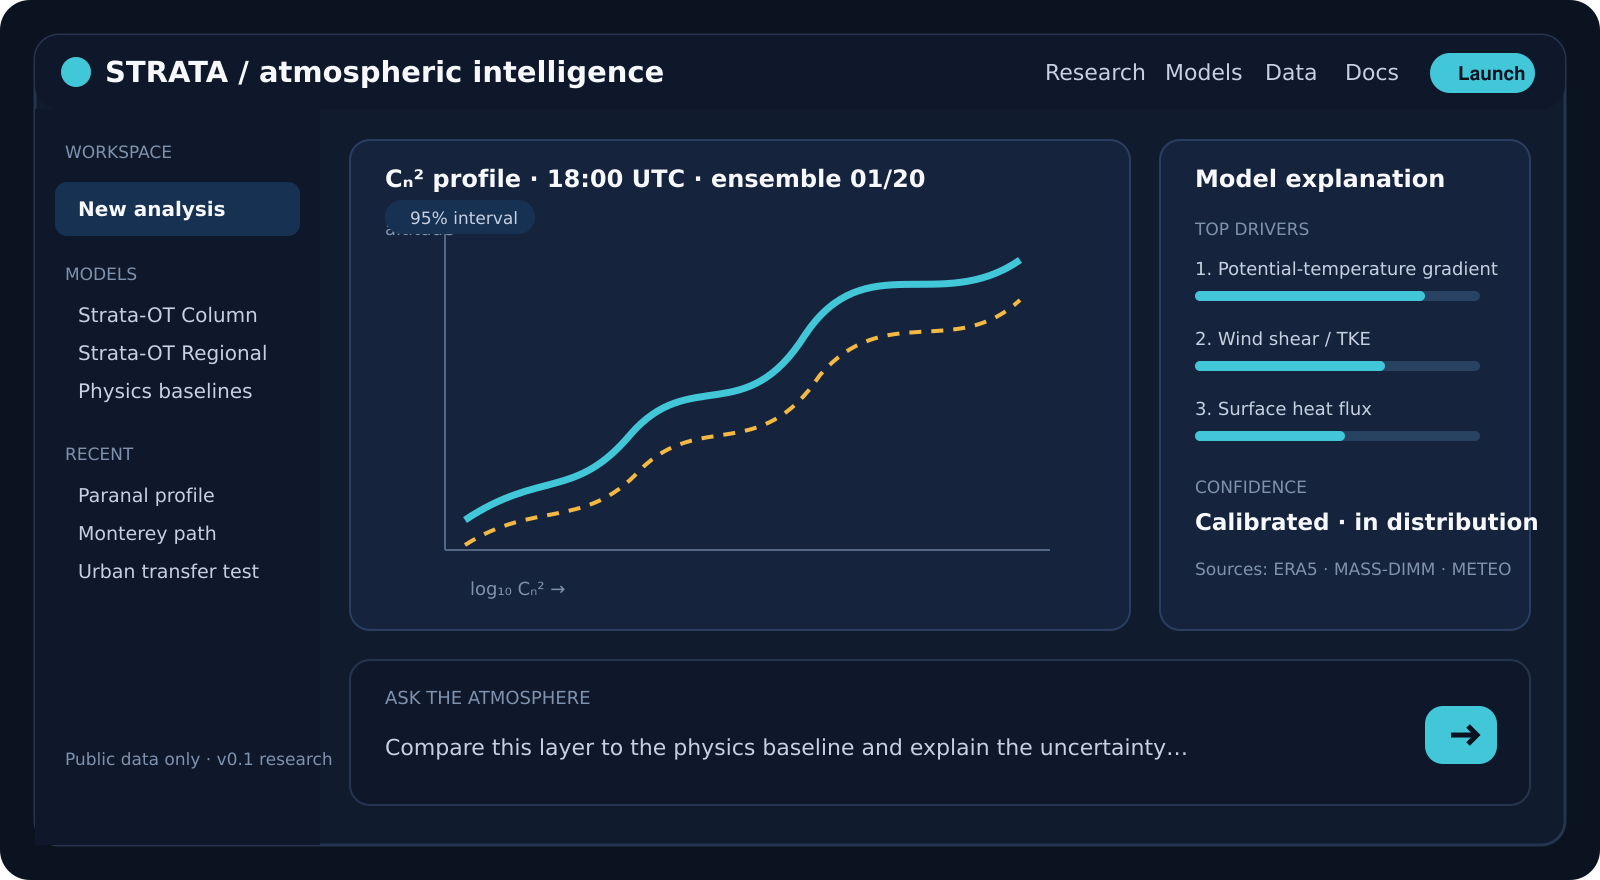
\includegraphics[width=\linewidth]{briefing-assets/media/f0d89ad15158a5ed2fe4f88a0d3429d3336ab8cf.png}

\textbf{Figure 2.} Concept for a research-first profile explorer with an
assistant layer, provenance and calibrated uncertainty.

\textbf{10.1 Public positioning}

\begin{longtable}[]{@{}
  >{\raggedright\arraybackslash}p{(\columnwidth - 2\tabcolsep) * \real{0.0218}}
  >{\raggedright\arraybackslash}p{(\columnwidth - 2\tabcolsep) * \real{0.9782}}@{}}
\toprule\noalign{}
\endhead
\bottomrule\noalign{}
\endlastfoot
& \textbf{SUGGESTED PUBLIC MESSAGE}

Open atmospheric intelligence for optical systems---profiles, forecasts,
benchmarks and tools for astronomy, free-space communications, imaging
and turbulence research. \\
\end{longtable}

Lead with broad scientific utility. Defense relevance can be
acknowledged in publications where cleared, but the public product
should not expose controlled integration details, system parameters,
operational test data or claims about weapon effectiveness.

\textbf{10.2 Information architecture}

\begin{longtable}[]{@{}
  >{\raggedright\arraybackslash}p{(\columnwidth - 4\tabcolsep) * \real{0.1816}}
  >{\raggedright\arraybackslash}p{(\columnwidth - 4\tabcolsep) * \real{0.3429}}
  >{\raggedright\arraybackslash}p{(\columnwidth - 4\tabcolsep) * \real{0.4754}}@{}}
\toprule\noalign{}
\begin{minipage}[b]{\linewidth}\raggedright
\textbf{Route}
\end{minipage} & \begin{minipage}[b]{\linewidth}\raggedright
\textbf{Purpose}
\end{minipage} & \begin{minipage}[b]{\linewidth}\raggedright
\textbf{Signature feature}
\end{minipage} \\
\midrule\noalign{}
\endhead
\bottomrule\noalign{}
\endlastfoot
/ & Research narrative and flagship model & Live profile animation with
uncertainty and one clear thesis \\
/playground & Interactive query / compare & Location, time,
altitude/path and model controls; natural-language analysis \\
/models & Family registry & Model cards, validated domains, calibration,
latency, weights and licenses \\
/data & Dataset catalog & Map, instrument geometry, coverage, quality,
license and downloadable schema \\
/benchmark & Transparent leaderboard & Fixed tasks, per-site results,
tail metrics, calibration and reproducible submissions \\
/research & Papers and technical reports & Readable paper pages with
figures, citations, code and DOI \\
/docs & API and SDK & Copyable Python/TypeScript examples and response
schemas \\
/safety-release & Boundaries and governance & Data provenance, known
limitations, public/controlled separation and review status \\
\end{longtable}

\textbf{10.3 Playground interaction model}

\begin{enumerate}
\def\labelenumi{\arabic{enumi}.}
\item
  \textbf{Specify atmosphere.} Choose location/time/forecast lead, load
  an example, or paste a path/vertical-column definition.
\item
  \textbf{Inspect prediction.} Plot median and ensemble Cn², highlight
  layers and show derived optical integrals with conventions.
\item
  \textbf{Compare evidence.} Overlay physics baseline, prior model
  version and any public observations; explain drivers and disagreement.
\item
  \textbf{Interrogate.} Ask an assistant why uncertainty rose, which
  variables mattered, or how the result changes under another
  model---answers cite model/data cards.
\item
  \textbf{Reproduce.} Export a signed JSON request/response, Python
  snippet, plot and provenance bundle.
\end{enumerate}

\textbf{10.4 Visual language}

\begin{itemize}
\item
  Near-black/navy canvas, cool cyan for predicted profiles, amber for
  physics baselines, restrained red only for OOD or invalid data.
\item
  Dense scientific plots with generous whitespace; monospaced numerals
  for coordinates and units.
\item
  Motion should reveal vertical evolution and uncertainty, never
  decorate static content.
\item
  Every result carries a visible model version, data timestamp,
  validated-domain badge and citation drawer.
\item
  Avoid mimicking OpenAI/Kimi/Claude logos, typography or page
  composition; borrow the interaction quality, not the brand.
\end{itemize}

\textbf{10.5 Technical stack}

\begin{longtable}[]{@{}
  >{\raggedright\arraybackslash}p{(\columnwidth - 2\tabcolsep) * \real{0.2244}}
  >{\raggedright\arraybackslash}p{(\columnwidth - 2\tabcolsep) * \real{0.7756}}@{}}
\toprule\noalign{}
\begin{minipage}[b]{\linewidth}\raggedright
\textbf{Layer}
\end{minipage} & \begin{minipage}[b]{\linewidth}\raggedright
\textbf{Recommendation}
\end{minipage} \\
\midrule\noalign{}
\endhead
\bottomrule\noalign{}
\endlastfoot
Web & Next.js/React + TypeScript; Tailwind or a small token system;
server-render research pages \\
Scientific visualization & Plotly/ECharts for profiles; MapLibre/deck.gl
for terrain and coverage; WebGL only where it adds value \\
API & FastAPI or gRPC-backed Python inference; versioned OpenAPI schemas
and signed provenance \\
Data & Object storage for Zarr/NetCDF, Parquet observation index,
Postgres metadata, cache for common queries \\
Models & PyTorch training; ONNX/TensorRT for Lite/Column inference where
validated; ensemble jobs asynchronous \\
Research search & Curated citation graph and retrieval index over
released papers/model cards; never mix controlled documents \\
Ops & Separate public and controlled accounts/networks; immutable model
artifacts, SBOMs, audit logs and release approvals \\
\end{longtable}

\textbf{10.6 Launch package}

\begin{itemize}
\item
  Preprint + archival DOI + plain-language technical report.
\item
  Weights, inference code, training configuration and exact benchmark
  commits where releasable.
\item
  Dataset cards and manifest even when raw data cannot be redistributed.
\item
  Interactive error atlas showing strong results and known failures.
\item
  Model card with intended uses, prohibited claims, calibrated domain,
  OOD behavior and licensing.
\item
  Public issue tracker, citation file, contribution guide and benchmark
  submission template.
\end{itemize}

\textbf{11. Security, release and dual-use boundaries}

\emph{A public atmospheric model can be broadly beneficial, while
defense-funded data, adapters and integration details may have separate
release obligations. Build that separation into the repository and
infrastructure from day one.}

\begin{longtable}[]{@{}
  >{\raggedright\arraybackslash}p{(\columnwidth - 2\tabcolsep) * \real{0.0218}}
  >{\raggedright\arraybackslash}p{(\columnwidth - 2\tabcolsep) * \real{0.9782}}@{}}
\toprule\noalign{}
\endhead
\bottomrule\noalign{}
\endlastfoot
& \textbf{NOT LEGAL ADVICE}

Contract, security and export counsel must classify each dataset, weight
file, interface and publication. Publicly available inputs do not
automatically make a defense-integrated artifact publicly releasable. \\
\end{longtable}

\textbf{11.1 Recommended two-track architecture}

\begin{longtable}[]{@{}
  >{\raggedright\arraybackslash}p{(\columnwidth - 2\tabcolsep) * \real{0.5000}}
  >{\raggedright\arraybackslash}p{(\columnwidth - 2\tabcolsep) * \real{0.5000}}@{}}
\toprule\noalign{}
\begin{minipage}[b]{\linewidth}\raggedright
\textbf{Public research core}
\end{minipage} & \begin{minipage}[b]{\linewidth}\raggedright
\textbf{Controlled / customer layer}
\end{minipage} \\
\midrule\noalign{}
\endhead
\bottomrule\noalign{}
\endlastfoot
Public observations and reanalysis; reproducible benchmark &
Contract/customer data, system-specific tests and operational
telemetry \\
Generic Cn² profile/forecast and uncertainty outputs & System adapters,
restricted geometries, mission-specific evaluation \\
Open physics baselines, weights and model cards after review &
Restricted weights, calibration parameters and interfaces \\
Public astronomy/FSO/imaging demos & Access-controlled integration and
validation environments \\
Public source papers and release-cleared results & CUI/export-controlled
or otherwise restricted technical information \\
\end{longtable}

\textbf{11.2 Release checklist}

\begin{itemize}
\item
  Confirm data ownership, redistribution terms, sponsor acknowledgments
  and derivative-data rights.
\item
  Determine whether the artifact contains official DoW/DoD information,
  CUI, export-controlled technical data, proprietary information or
  contract restrictions.
\item
  Use the responsible security/prepublication channel before posting
  defense-related manuscripts, talks, websites, code or model artifacts.
\item
  Review model weights as technical artifacts; do not assume only source
  code and documents require classification/export analysis.
\item
  Keep public infrastructure free of controlled prompts, logs, papers,
  embeddings and telemetry.
\item
  Record release authority, version, hash and approved scope for every
  public artifact.
\item
  Avoid performance claims outside validated public datasets and clearly
  mark simulator-derived results.
\end{itemize}

Authoritative starting points:
\href{https://www.esd.whs.mil/Records-Declass/Security-Review/PrePublication-and-Manuscripts/}{\ul{DOPSR
public-release guidance}} ·
\href{https://www.bis.gov/regulations/ear/734}{\ul{EAR Part 734}} ·
\href{https://www.pmddtc.state.gov/ddtc_public?id=ddtc_public_portal_itar_landing}{\ul{DDTC
ITAR overview}}

\textbf{12. Recommendations and 30-day start}

\emph{The right first month proves that the benchmark is real, the data
are legally usable, and the claimed baselines can be reproduced.
Architecture work should begin in parallel but cannot outrun those
facts.}

\textbf{12.1 Decisions}

\begin{longtable}[]{@{}
  >{\raggedright\arraybackslash}p{(\columnwidth - 2\tabcolsep) * \real{0.2778}}
  >{\raggedright\arraybackslash}p{(\columnwidth - 2\tabcolsep) * \real{0.7222}}@{}}
\toprule\noalign{}
\begin{minipage}[b]{\linewidth}\raggedright
\textbf{Decision}
\end{minipage} & \begin{minipage}[b]{\linewidth}\raggedright
\textbf{Recommendation}
\end{minipage} \\
\midrule\noalign{}
\endhead
\bottomrule\noalign{}
\endlastfoot
Proceed? & Yes---phase-gated research program. \\
First flagship? & Strata-OT Column, not a billion-parameter regional
model. \\
Primary novelty? & Physics latent state + heterogeneous observation
operators + extreme-aware probabilistic residual. \\
Primary moat? & OpenCn2 schema, multisite benchmark, instrument metadata
and controlled field partnerships. \\
First public product? & Benchmark/error atlas and profile playground
with honest uncertainty. \\
Open strategy? & Open public atmospheric core after review; separate
restricted adapters/data/integration. \\
\end{longtable}

\textbf{12.2 Thirty-day build plan}

\begin{enumerate}
\def\labelenumi{\arabic{enumi}.}
\item
  \textbf{Days 1--3: repository and governance.} Create public/private
  boundaries, data license register, model registry and experiment
  template.
\item
  \textbf{Days 1--10: reproduce.} Run otbench MLO/USNA tasks,
  reimplement physics baselines and reproduce one neural result with
  frozen time splits.
\item
  \textbf{Days 4--14: acquire and normalize.} Ingest OTProf, ESO and
  approved TMT subsets; write geometry-aware common records and QC
  reports.
\item
  \textbf{Days 8--18: build model skeleton.} Column encoder, continuous
  coordinate decoder, uncertainty head and differentiable point/path
  operators.
\item
  \textbf{Days 15--24: train v0.} Teacher pretraining on OTProf,
  fine-tune on MLO/USNA, then evaluate blocked time and leave-dataset
  transfer.
\item
  \textbf{Days 20--27: error atlas.} Break results down by hour,
  stability, wind sector, altitude, instrument and Cn² quantile; find
  leakage and smoothing.
\item
  \textbf{Days 24--30: public prototype.} Static research site shell,
  model/data cards and a prerecorded or cached profile demo using public
  data only.
\end{enumerate}

\textbf{12.3 The first demo that will impress experts}

\begin{longtable}[]{@{}
  >{\raggedright\arraybackslash}p{(\columnwidth - 2\tabcolsep) * \real{0.0218}}
  >{\raggedright\arraybackslash}p{(\columnwidth - 2\tabcolsep) * \real{0.9782}}@{}}
\toprule\noalign{}
\endhead
\bottomrule\noalign{}
\endlastfoot
& \textbf{DEMO}

Select a withheld site and date. Show the predicted Cn² profile ensemble
evolving through a boundary-layer transition, overlay the physics
baseline and observations, identify the dominant layer, display
calibrated r₀/seeing consequences, explain the top physical drivers, and
expose the exact data/model provenance. Then switch to an unseen site
and let the OOD indicator become visibly honest. \\
\end{longtable}

\textbf{12.4 Final judgment}

\textbf{This is worth building.} The field now has enough open data,
modern precedent and cross-domain architecture evidence for a serious
model family. The winning program will resist the temptation to market
same-site interpolation as a universal solution. If the benchmark,
observation physics and uncertainty are built first, Strata-OT can be
both technically credible and visually compelling.

\textbf{Appendix A. Detailed dataset acquisition cards}

\emph{Priority order reflects value for a first public benchmark, not
intrinsic scientific importance.}

\textbf{A.1 otbench: MLO\_Cn2 + USNA Cn² tasks}

\begin{longtable}[]{@{}
  >{\raggedright\arraybackslash}p{(\columnwidth - 2\tabcolsep) * \real{0.1603}}
  >{\raggedright\arraybackslash}p{(\columnwidth - 2\tabcolsep) * \real{0.8397}}@{}}
\toprule\noalign{}
\begin{minipage}[b]{\linewidth}\raggedright
\textbf{Field}
\end{minipage} & \begin{minipage}[b]{\linewidth}\raggedright
\textbf{Detail}
\end{minipage} \\
\midrule\noalign{}
\endhead
\bottomrule\noalign{}
\endlastfoot
Priority & A \\
Label & Direct surface / path-averaged Cn² + meteorology \\
Scale & Multiple benchmark tasks; regression and forecast splits \\
Access & Open code/data loader; MIT package \\
Best use & First reproducible benchmark and baselines \\
Main risk & Few environments; inspect task licenses and missingness \\
Source &
\href{https://github.com/CDJellen/otbench}{\ul{https://github.com/CDJellen/otbench}} \\
\end{longtable}

\textbf{A.2 NCAR MLO\_CN2}

\begin{longtable}[]{@{}
  >{\raggedright\arraybackslash}p{(\columnwidth - 2\tabcolsep) * \real{0.1603}}
  >{\raggedright\arraybackslash}p{(\columnwidth - 2\tabcolsep) * \real{0.8397}}@{}}
\toprule\noalign{}
\begin{minipage}[b]{\linewidth}\raggedright
\textbf{Field}
\end{minipage} & \begin{minipage}[b]{\linewidth}\raggedright
\textbf{Detail}
\end{minipage} \\
\midrule\noalign{}
\endhead
\bottomrule\noalign{}
\endlastfoot
Priority & A \\
Label & High-rate sonic-derived surface-layer turbulence \\
Scale & 9 Jun--8 Aug 2006, Mauna Loa \\
Access & Open NCAR/EOL archive \\
Best use & Few-shot, local transfer and surface physics \\
Main risk & Single high-altitude dry site; short campaign \\
Source &
\href{https://www.eol.ucar.edu/field_projects/mlocn2}{\ul{https://www.eol.ucar.edu/field\_projects/mlocn2}} \\
\end{longtable}

\textbf{A.3 TMT Site Testing Database}

\begin{longtable}[]{@{}
  >{\raggedright\arraybackslash}p{(\columnwidth - 2\tabcolsep) * \real{0.1603}}
  >{\raggedright\arraybackslash}p{(\columnwidth - 2\tabcolsep) * \real{0.8397}}@{}}
\toprule\noalign{}
\begin{minipage}[b]{\linewidth}\raggedright
\textbf{Field}
\end{minipage} & \begin{minipage}[b]{\linewidth}\raggedright
\textbf{Detail}
\end{minipage} \\
\midrule\noalign{}
\endhead
\bottomrule\noalign{}
\endlastfoot
Priority & A \\
Label & MASS/DIMM, SODAR, weather, sonic; profile/integrated products \\
Scale & Five candidate sites, roughly 2--5 years \\
Access & Free with login and publication conditions \\
Best use & Leave-one-site-out profile and instrument transfer \\
Main risk & Data intentionally unfiltered; rigorous QC required \\
Source &
\href{https://sitedata.tmt.org/}{\ul{https://sitedata.tmt.org/}} \\
\end{longtable}

\textbf{A.4 ESO Paranal Ambient / ASM}

\begin{longtable}[]{@{}
  >{\raggedright\arraybackslash}p{(\columnwidth - 2\tabcolsep) * \real{0.1603}}
  >{\raggedright\arraybackslash}p{(\columnwidth - 2\tabcolsep) * \real{0.8397}}@{}}
\toprule\noalign{}
\begin{minipage}[b]{\linewidth}\raggedright
\textbf{Field}
\end{minipage} & \begin{minipage}[b]{\linewidth}\raggedright
\textbf{Detail}
\end{minipage} \\
\midrule\noalign{}
\endhead
\bottomrule\noalign{}
\endlastfoot
Priority & A \\
Label & DIMM Cn²/seeing, MASS 6-layer profile, SLODAR surface layer,
met \\
Scale & DIMM since 1998; MASS since 2016; SLODAR 2016--2020 \\
Access & Open query/download interface \\
Best use & Long temporal holdouts, profile + integrated multitask
learning \\
Main risk & Astronomical line-of-sight and nighttime selection
effects \\
Source &
\href{https://archive.eso.org/wdb/help/eso/ambient_paranal.html}{\ul{https://archive.eso.org/wdb/help/eso/ambient\_paranal.html}} \\
\end{longtable}

\textbf{A.5 OTProf WRF--ERA5 corpus}

\begin{longtable}[]{@{}
  >{\raggedright\arraybackslash}p{(\columnwidth - 2\tabcolsep) * \real{0.1603}}
  >{\raggedright\arraybackslash}p{(\columnwidth - 2\tabcolsep) * \real{0.8397}}@{}}
\toprule\noalign{}
\begin{minipage}[b]{\linewidth}\raggedright
\textbf{Field}
\end{minipage} & \begin{minipage}[b]{\linewidth}\raggedright
\textbf{Detail}
\end{minipage} \\
\midrule\noalign{}
\endhead
\bottomrule\noalign{}
\endlastfoot
Priority & A− \\
Label & Teacher Cn² profiles + TKE, θ variance and length scale \\
Scale & 25.7 GB; paired high-/coarse-resolution columns \\
Access & Open Zenodo + code \\
Best use & Pretraining, profile decoder reproduction, architecture
baseline \\
Main risk & Synthetic teacher bias; not independent ground truth \\
Source &
\href{https://doi.org/10.5281/zenodo.20733692}{\ul{https://doi.org/10.5281/zenodo.20733692}} \\
\end{longtable}

\textbf{A.6 WRF Cn² parameterization intercomparison}

\begin{longtable}[]{@{}
  >{\raggedright\arraybackslash}p{(\columnwidth - 2\tabcolsep) * \real{0.1603}}
  >{\raggedright\arraybackslash}p{(\columnwidth - 2\tabcolsep) * \real{0.8397}}@{}}
\toprule\noalign{}
\begin{minipage}[b]{\linewidth}\raggedright
\textbf{Field}
\end{minipage} & \begin{minipage}[b]{\linewidth}\raggedright
\textbf{Detail}
\end{minipage} \\
\midrule\noalign{}
\endhead
\bottomrule\noalign{}
\endlastfoot
Priority & B+ \\
Label & Post-processed WRF and meteorology; parameterization outputs \\
Scale & Two study sites / cases \\
Access & Open Zenodo + GitHub \\
Best use & Physics teacher and parameterization benchmark \\
Main risk & Scintillometer validation labels withheld \\
Source &
\href{https://doi.org/10.5281/zenodo.10966120}{\ul{https://doi.org/10.5281/zenodo.10966120}} \\
\end{longtable}

\textbf{A.7 Turbulence Strength Dataset (video + scintillometer)}

\begin{longtable}[]{@{}
  >{\raggedright\arraybackslash}p{(\columnwidth - 2\tabcolsep) * \real{0.1603}}
  >{\raggedright\arraybackslash}p{(\columnwidth - 2\tabcolsep) * \real{0.8397}}@{}}
\toprule\noalign{}
\begin{minipage}[b]{\linewidth}\raggedright
\textbf{Field}
\end{minipage} & \begin{minipage}[b]{\linewidth}\raggedright
\textbf{Detail}
\end{minipage} \\
\midrule\noalign{}
\endhead
\bottomrule\noalign{}
\endlastfoot
Priority & B \\
Label & Images synchronized to path-averaged Cn² \\
Scale & Two Arizona sets, \textasciitilde30k images each \\
Access & Public download + code \\
Best use & Observation encoder and multimodal proof of concept \\
Main risk & Only \textasciitilde5.75 hours, fixed scenes and daytime
illumination \\
Source &
\href{https://github.com/Riponcs/TurbulenceDataset}{\ul{https://github.com/Riponcs/TurbulenceDataset}} \\
\end{longtable}

\textbf{A.8 CASES-99 high-rate surface flux data}

\begin{longtable}[]{@{}
  >{\raggedright\arraybackslash}p{(\columnwidth - 2\tabcolsep) * \real{0.1603}}
  >{\raggedright\arraybackslash}p{(\columnwidth - 2\tabcolsep) * \real{0.8397}}@{}}
\toprule\noalign{}
\begin{minipage}[b]{\linewidth}\raggedright
\textbf{Field}
\end{minipage} & \begin{minipage}[b]{\linewidth}\raggedright
\textbf{Detail}
\end{minipage} \\
\midrule\noalign{}
\endhead
\bottomrule\noalign{}
\endlastfoot
Priority & B \\
Label & 20-Hz 3-D sonic winds and fast scalar variables \\
Scale & Main tower + six stations; stable boundary layer \\
Access & Open NCAR/EOL NetCDF \\
Best use & Derive C\_T² / stability labels and pretrain turbulence
encoders \\
Main risk & Derived rather than optical label; sensor/QC expertise
required \\
Source &
\href{https://www.eol.ucar.edu/content/sample-rate-isff-data-cases99}{\ul{https://www.eol.ucar.edu/content/sample-rate-isff-data-cases99}} \\
\end{longtable}

\textbf{A.9 MATERHORN-X}

\begin{longtable}[]{@{}
  >{\raggedright\arraybackslash}p{(\columnwidth - 2\tabcolsep) * \real{0.1603}}
  >{\raggedright\arraybackslash}p{(\columnwidth - 2\tabcolsep) * \real{0.8397}}@{}}
\toprule\noalign{}
\begin{minipage}[b]{\linewidth}\raggedright
\textbf{Field}
\end{minipage} & \begin{minipage}[b]{\linewidth}\raggedright
\textbf{Detail}
\end{minipage} \\
\midrule\noalign{}
\endhead
\bottomrule\noalign{}
\endlastfoot
Priority & B \\
Label & Dense mountain meteorology and turbulence observations \\
Scale & Dry, fall, spring and fog campaigns \\
Access & NCAR/EOL archive \\
Best use & Complex-terrain representation and regime stress tests \\
Main risk & Cn² must be derived or paired with a physics teacher \\
Source &
\href{https://www.eol.ucar.edu/field_projects/materhorn-x}{\ul{https://www.eol.ucar.edu/field\_projects/materhorn-x}} \\
\end{longtable}

\textbf{A.10 Perdigão 2017}

\begin{longtable}[]{@{}
  >{\raggedright\arraybackslash}p{(\columnwidth - 2\tabcolsep) * \real{0.1603}}
  >{\raggedright\arraybackslash}p{(\columnwidth - 2\tabcolsep) * \real{0.8397}}@{}}
\toprule\noalign{}
\begin{minipage}[b]{\linewidth}\raggedright
\textbf{Field}
\end{minipage} & \begin{minipage}[b]{\linewidth}\raggedright
\textbf{Detail}
\end{minipage} \\
\midrule\noalign{}
\endhead
\bottomrule\noalign{}
\endlastfoot
Priority & B \\
Label & Dense sonic, mast, lidar and energy-balance observations \\
Scale & Two-ridge complex terrain; Dec 2016--Jun 2017 \\
Access & NCAR/EOL archive \\
Best use & Terrain-aware encoders and multiscale turbulence
pretraining \\
Main risk & No direct optical label \\
Source &
\href{https://www.eol.ucar.edu/field_projects/perdig\%C3\%A3o}{\ul{https://www.eol.ucar.edu/field\_projects/perdig\%C3\%A3o}} \\
\end{longtable}

\textbf{A.11 ERA5 / ERA5-Land}

\begin{longtable}[]{@{}
  >{\raggedright\arraybackslash}p{(\columnwidth - 2\tabcolsep) * \real{0.1603}}
  >{\raggedright\arraybackslash}p{(\columnwidth - 2\tabcolsep) * \real{0.8397}}@{}}
\toprule\noalign{}
\begin{minipage}[b]{\linewidth}\raggedright
\textbf{Field}
\end{minipage} & \begin{minipage}[b]{\linewidth}\raggedright
\textbf{Detail}
\end{minipage} \\
\midrule\noalign{}
\endhead
\bottomrule\noalign{}
\endlastfoot
Priority & A covariate \\
Label & Global atmospheric covariates, pressure levels and surface
fields \\
Scale & Hourly, multidecadal global coverage \\
Access & Open via Copernicus CDS terms \\
Best use & Foundation pretraining, historical covariates and
climatology \\
Main risk & Coarse boundary layer and terrain; not a Cn² label \\
Source &
\href{https://cds.climate.copernicus.eu/datasets/reanalysis-era5-pressure-levels}{\ul{https://cds.climate.copernicus.eu/datasets/reanalysis-era5-pressure-levels}} \\
\end{longtable}

\textbf{A.12 NOAA HRRR}

\begin{longtable}[]{@{}
  >{\raggedright\arraybackslash}p{(\columnwidth - 2\tabcolsep) * \real{0.1603}}
  >{\raggedright\arraybackslash}p{(\columnwidth - 2\tabcolsep) * \real{0.8397}}@{}}
\toprule\noalign{}
\begin{minipage}[b]{\linewidth}\raggedright
\textbf{Field}
\end{minipage} & \begin{minipage}[b]{\linewidth}\raggedright
\textbf{Detail}
\end{minipage} \\
\midrule\noalign{}
\endhead
\bottomrule\noalign{}
\endlastfoot
Priority & A covariate \\
Label & 3-km hourly analyses/forecasts with rich boundary-layer
fields \\
Scale & CONUS archive since 2014 \\
Access & Open cloud archive \\
Best use & Higher-resolution U.S. covariates and forecast-time
realism \\
Main risk & Model changes and archive volume; no direct Cn² \\
Source &
\href{https://registry.opendata.aws/noaa-hrrr-pds/}{\ul{https://registry.opendata.aws/noaa-hrrr-pds/}} \\
\end{longtable}

\textbf{A.13 New York State Mesonet}

\begin{longtable}[]{@{}
  >{\raggedright\arraybackslash}p{(\columnwidth - 2\tabcolsep) * \real{0.1603}}
  >{\raggedright\arraybackslash}p{(\columnwidth - 2\tabcolsep) * \real{0.8397}}@{}}
\toprule\noalign{}
\begin{minipage}[b]{\linewidth}\raggedright
\textbf{Field}
\end{minipage} & \begin{minipage}[b]{\linewidth}\raggedright
\textbf{Detail}
\end{minipage} \\
\midrule\noalign{}
\endhead
\bottomrule\noalign{}
\endlastfoot
Priority & B+ \\
Label & 5-min surface meteorology; flux network at selected stations \\
Scale & 127 stations; 17 used by OTCliM \\
Access & Data request / terms vary by use \\
Best use & Near-surface cross-site benchmark and urban/rural regimes \\
Main risk & Access and redistribution constraints; Cn² subset
provenance \\
Source & \href{https://nysmesonet.org/}{\ul{https://nysmesonet.org/}} \\
\end{longtable}

\textbf{A.14 OCAN g-SCIDAR profile archive}

\begin{longtable}[]{@{}
  >{\raggedright\arraybackslash}p{(\columnwidth - 2\tabcolsep) * \real{0.1603}}
  >{\raggedright\arraybackslash}p{(\columnwidth - 2\tabcolsep) * \real{0.8397}}@{}}
\toprule\noalign{}
\begin{minipage}[b]{\linewidth}\raggedright
\textbf{Field}
\end{minipage} & \begin{minipage}[b]{\linewidth}\raggedright
\textbf{Detail}
\end{minipage} \\
\midrule\noalign{}
\endhead
\bottomrule\noalign{}
\endlastfoot
Priority & A if licensed \\
Label & High-resolution vertical Cn² profiles \\
Scale & Nearly 300 nights; hundreds of thousands of profiles \\
Access & Paper public; database access not established \\
Best use & Potential profile foundation corpus / external
collaboration \\
Main risk & Gated or author-mediated; observatory/nighttime domain \\
Source &
\href{https://arxiv.org/abs/2607.25940}{\ul{https://arxiv.org/abs/2607.25940}} \\
\end{longtable}

\textbf{A.15 Chesapeake Bay neural scintillometry corpus}

\begin{longtable}[]{@{}
  >{\raggedright\arraybackslash}p{(\columnwidth - 2\tabcolsep) * \real{0.1603}}
  >{\raggedright\arraybackslash}p{(\columnwidth - 2\tabcolsep) * \real{0.8397}}@{}}
\toprule\noalign{}
\begin{minipage}[b]{\linewidth}\raggedright
\textbf{Field}
\end{minipage} & \begin{minipage}[b]{\linewidth}\raggedright
\textbf{Detail}
\end{minipage} \\
\midrule\noalign{}
\endhead
\bottomrule\noalign{}
\endlastfoot
Priority & A if licensed \\
Label & Pupil-plane imagery + path Cn² + air--water temperature
difference \\
Scale & \textgreater12 million images, 16.2 km, nearly five months \\
Access & Paper open; corpus availability not stated \\
Best use & Large-scale optical encoder and instrument modeling \\
Main risk & Requires partnership; one maritime path/instrument \\
Source &
\href{https://opg.optica.org/ao/abstract.cfm?uri=ao-65-19-H86}{\ul{https://opg.optica.org/ao/abstract.cfm?uri=ao-65-19-H86}} \\
\end{longtable}

\textbf{A.16 On-demand WRF / LES / phase-screen generation}

\begin{longtable}[]{@{}
  >{\raggedright\arraybackslash}p{(\columnwidth - 2\tabcolsep) * \real{0.1603}}
  >{\raggedright\arraybackslash}p{(\columnwidth - 2\tabcolsep) * \real{0.8397}}@{}}
\toprule\noalign{}
\begin{minipage}[b]{\linewidth}\raggedright
\textbf{Field}
\end{minipage} & \begin{minipage}[b]{\linewidth}\raggedright
\textbf{Detail}
\end{minipage} \\
\midrule\noalign{}
\endhead
\bottomrule\noalign{}
\endlastfoot
Priority & Teacher only \\
Label & Synthetic latent physics, Cn² teachers and optical
observables \\
Scale & Controllable, effectively unlimited \\
Access & Open software; compute- and expertise-intensive \\
Best use & Coverage of rare regimes, pretraining and controlled
ablations \\
Main risk & Simulation bias must never be confused with field truth \\
Source &
\href{https://www2.mmm.ucar.edu/wrf/users/}{\ul{https://www2.mmm.ucar.edu/wrf/users/}} \\
\end{longtable}

\textbf{Appendix B. Experiment backlog}

\emph{A deliberately broad backlog for ablation planning, student
projects and follow-on papers.}

\begin{longtable}[]{@{}
  >{\raggedright\arraybackslash}p{(\columnwidth - 4\tabcolsep) * \real{0.1282}}
  >{\raggedright\arraybackslash}p{(\columnwidth - 4\tabcolsep) * \real{0.4776}}
  >{\raggedright\arraybackslash}p{(\columnwidth - 4\tabcolsep) * \real{0.3942}}@{}}
\toprule\noalign{}
\begin{minipage}[b]{\linewidth}\raggedright
\textbf{Theme}
\end{minipage} & \begin{minipage}[b]{\linewidth}\raggedright
\textbf{Experiment}
\end{minipage} & \begin{minipage}[b]{\linewidth}\raggedright
\textbf{Question answered}
\end{minipage} \\
\midrule\noalign{}
\endhead
\bottomrule\noalign{}
\endlastfoot
Data & Instrument-bias embeddings vs explicit calibration correction &
Transfer across scintillometers / observatories \\
Data & CF-height vs pressure vs geopotential vertical coordinates &
Profile fidelity and cross-terrain transfer \\
Data & Quantile mapping of ERA5/HRRR to WRF distributions &
Teacher/inference covariate mismatch \\
Data & Raw vs QC-filtered vs uncertainty-weighted labels & Robustness to
noisy direct observations \\
Data & Campaign-balanced vs sample-balanced batches & Prevent long
campaigns dominating \\
Pretraining & Masked levels, channels and time windows & Best
atmospheric representation objective \\
Pretraining & ERA5 only vs ERA5+HRRR vs multi-NWP & Transfer and
model-version robustness \\
Pretraining & Predict θ variance/TKE/ε vs reconstruct weather only &
Turbulence-aware features \\
Architecture & 1-D Squeezeformer vs vertical neural operator &
Continuous resolution and sharp layers \\
Architecture & AFNO/FNO vs local attention vs terrain graph & Regional
efficiency and complex-terrain skill \\
Architecture & Perceiver sensor tokens vs Set Transformer & Irregular
observation assimilation \\
Architecture & Soft environment experts vs single backbone &
Worst-regime performance \\
Architecture & Boundary/free-atmosphere split height fixed vs learned &
Stable layer and entrainment behavior \\
Physics & Direct Cn² vs C\_T²/C\_q²/C\_Tq decoder & Humidity-aware
transfer \\
Physics & Cholesky covariance vs penalty constraints & Numerical
stability and physical validity \\
Physics & Variance-based teacher vs multi-parameterization ensemble &
Teacher bias reduction \\
Physics & Learned residual around physics vs full neural prediction &
Few-shot and OOD behavior \\
Output & Fixed levels vs continuous coordinate queries &
Super-resolution and arbitrary paths \\
Output & Lognormal NLL vs Student-t vs mixture density & Heavy-tail
calibration \\
Output & Quantile head vs conditional flow vs diffusion & Extreme layers
and sampling cost \\
Output & Vertical derivative/spectral loss & Layer sharpness without
hallucination \\
Sampling & Quantile-balanced / event-balanced sampling & Rare strong
turbulence recall \\
Sampling & Sunrise/sunset transition curriculum & Rapid regime shift
performance \\
Assimilation & One-day context set vs LoRA fine-tune & Fast site
adaptation \\
Assimilation & Posterior update with/without instrument identity &
Sensor calibration and uncertainty \\
Uncertainty & Deep ensemble vs single-model flow ensembles &
Epistemic/aleatoric separation \\
Uncertainty & Conformal intervals by regime & Finite-sample coverage
under heterogeneity \\
OOD & Latent density vs energy score vs ensemble disagreement &
Selective prediction and fallback \\
Evaluation & Random split vs blocked split audit & Quantify leakage
inflation \\
Evaluation & Leave site vs leave instrument vs leave climate & Locate
source of domain shift \\
Evaluation & Profile metrics vs integrated optics metrics & Detect
smoothing-induced optimism \\
Evaluation & Worst-site objective / distributionally robust training &
Avoid average-score masking \\
Sensor & Video physics-CNN as observation token & Cheap passive local
updates \\
Sensor & Pupil-plane CNN pretraining then meteorological fusion & Neural
scintillometry generalization \\
Sensor & MASS/DIMM/SLODAR joint vertical response learning & Profile
resolution and instrument fusion \\
Regional & Independent columns vs spatial operator & Value of horizontal
context \\
Regional & Terrain graph at 30--100 m nested in 3-km NWP &
Boundary-layer downscaling \\
Regional & Coastline/wake directional features & Near-maritime and
land--sea interface skill \\
Generative & Phase screens conditioned on latent scales and profile &
Downstream statistical consistency \\
Product & Natural-language explanation grounded in model card &
Usability without unsupported claims \\
\end{longtable}

\textbf{Appendix C. Website content checklist}

\begin{longtable}[]{@{}
  >{\raggedright\arraybackslash}p{(\columnwidth - 2\tabcolsep) * \real{0.2244}}
  >{\raggedright\arraybackslash}p{(\columnwidth - 2\tabcolsep) * \real{0.7756}}@{}}
\toprule\noalign{}
\begin{minipage}[b]{\linewidth}\raggedright
\textbf{Artifact}
\end{minipage} & \begin{minipage}[b]{\linewidth}\raggedright
\textbf{Required content}
\end{minipage} \\
\midrule\noalign{}
\endhead
\bottomrule\noalign{}
\endlastfoot
Model card & Architecture, data summary, intended use, validated
domains, metrics by site/regime, uncertainty, OOD, limitations, license,
release authority \\
Dataset card & Source/owner, license, instrument, geometry, date/site
coverage, QC, missingness, transformations, known bias, allowed
redistribution \\
Benchmark card & Task definition, split hash, target, inputs allowed at
inference, metrics, baselines, leakage tests and submission format \\
Paper page & Abstract, key figures, methods, result tables,
code/data/model links, citation export, corrections and version
history \\
Prediction bundle & Request, model/version/hash, source timestamps,
units/conventions, ensemble summaries, OOD status and warnings \\
Leaderboard & Per-site and aggregate scores, confidence intervals,
compute/latency, reproducibility status and external validation badge \\
Release record & Approval scope/date, artifact hashes, license/SBOM,
responsible contact and withdrawal/update mechanism \\
\end{longtable}

\textbf{Appendix D. Bibliography and discovery corpus}

\emph{The first list contains the recent and cross-domain sources used
to extend the 2025 review. The second carries forward that review's
167-item bibliography as a comprehensive discovery index. Verify primary
texts, licenses and current versions before publication or
implementation.}

\textbf{D.1 Recent and cross-domain additions}

\textbf{{[}1{]}} Quatresooz, F., and Oestges, C. (2025). Cn² Modeling
for Free-Space Optical Communications: A Review. IEEE Access 13,
21279--21305. https://doi.org/10.1109/ACCESS.2025.3535093

\textbf{{[}2{]}} Pierzyna, M., Basu, S., and Saathof, R. (2026). OTProf:
estimating high-resolution profiles of optical turbulence (Cn²) from
reanalysis using deep learning. arXiv:2604.09346.
https://arxiv.org/abs/2604.09346

\textbf{{[}3{]}} Pierzyna, M. (2026). Dataset: OTProf. Zenodo.
https://doi.org/10.5281/zenodo.20733692

\textbf{{[}4{]}} Basu, S. (2026). Leveraging deep learning-based
foundation models for optical turbulence (Cn²) estimation under data
scarcity. Applied Optics 65, 2497--2504.
https://doi.org/10.1364/AO.585045

\textbf{{[}5{]}} Bass, J. M., Singh, A. M., Mahon, R., and Ferraro, M.
S. (2026). Estimating atmospheric Cn² using deep convolutional neural
networks. Applied Optics 65(19), H86--H94.
https://opg.optica.org/ao/abstract.cfm?uri=ao-65-19-H86

\textbf{{[}6{]}} Hou, J., et al. (2026). Data-driven learning of
atmospheric turbulence phase screens via diffusion models. Applied
Optics 65, 4525.
https://opg.optica.org/ao/abstract.cfm?uri=ao-65-13-4525

\textbf{{[}7{]}} Salas, A., García-Lorenzo, B., Castro-Almazán, J. A.,
and Trancho, G. (2026). CNN-Based Reanalysis of Optical Turbulence at
the Canary Islands Observatories (OCAN). arXiv:2607.25940.
https://arxiv.org/abs/2607.25940

\textbf{{[}8{]}} Celik, U., Yasar, H. A., Keskin, M. Y., Bayar, C.,
Aslantas, I., and Midilli, Y. (2024). Estimation of ground-based
atmospheric turbulence strength (Cn²) by neural network architecture.
Applied Optics 63, 7402--7409. https://doi.org/10.1364/AO.532723

\textbf{{[}9{]}} Pierzyna, M., Hartogensis, O., Basu, S., and Saathof,
R. (2024). Intercomparison of flux-, gradient-, and variance-based
optical turbulence parameterizations. Applied Optics 63, E107--E119.
https://opg.optica.org/ao/abstract.cfm?uri=ao-63-16-E107

\textbf{{[}10{]}} Pierzyna, M., Basu, S., and Saathof, R. (2025).
OTCliM: generating a near-surface climatology of optical turbulence
strength using gradient boosting. Artificial Intelligence for the Earth
Systems 4(2).
https://journals.ametsoc.org/view/journals/aies/4/2/AIES-D-24-0076.1.xml

\textbf{{[}11{]}} Jellen, C., Nelson, C., Brownell, C., and Burkhardt,
J. (2024). Effective Benchmarks for Optical Turbulence Modeling.
Artificial Intelligence for the Earth Systems 3(4).
https://arxiv.org/abs/2401.03573

\textbf{{[}12{]}} Saha, R. K., Salcin, E., Kim, J., Smith, J., and
Jayasuriya, S. (2024). Turbulence Strength Cn² Estimation from Video
using Physics-based Deep Learning. arXiv:2408.16623.
https://arxiv.org/abs/2408.16623

\textbf{{[}13{]}} Basu, S., and Holtslag, A. A. M. (2022). Revisiting
and revising Tatarskii's formulation for the temperature structure
parameter in atmospheric flows. Environmental Fluid Mechanics.
https://doi.org/10.1007/s10652-022-09880-3

\textbf{{[}14{]}} Li, Z., Kovachki, N., Azizzadenesheli, K., et al.
(2021). Fourier Neural Operator for Parametric Partial Differential
Equations. ICLR. https://arxiv.org/abs/2010.08895

\textbf{{[}15{]}} Lu, L., Jin, P., Pang, G., Zhang, Z., and Karniadakis,
G. E. (2021). Learning nonlinear operators via DeepONet. Nature Machine
Intelligence 3, 218--229. https://doi.org/10.1038/s42256-021-00302-5

\textbf{{[}16{]}} Mardani, M., Brenowitz, N., Cohen, Y., et al. (2025).
Residual corrective diffusion modeling for km-scale atmospheric
downscaling. Communications Earth \& Environment 6.
https://doi.org/10.1038/s43247-025-02042-5

\textbf{{[}17{]}} Bodnar, C., Bruinsma, W. P., Lucic, A., et al. (2025).
A foundation model for the Earth system. Nature.
https://doi.org/10.1038/s41586-025-09005-y

\textbf{{[}18{]}} Kochkov, D., Yuval, J., Langmore, I., et al. (2024).
Neural general circulation models for weather and climate. Nature 632,
1060--1066. https://doi.org/10.1038/s41586-024-07744-y

\textbf{{[}19{]}} Bi, K., Xie, L., Zhang, H., et al. (2023). Accurate
medium-range global weather forecasting with 3D neural networks
(Pangu-Weather). Nature 619, 533--538.
https://doi.org/10.1038/s41586-023-06185-3

\textbf{{[}20{]}} Price, I., Sanchez-Gonzalez, A., Alet, F., et al.
(2025). Probabilistic weather forecasting with machine learning
(GenCast). Nature 637, 84--90.
https://doi.org/10.1038/s41586-024-08252-9

\textbf{{[}21{]}} Lam, R., Sanchez-Gonzalez, A., Willson, M., et al.
(2023). Learning skillful medium-range global weather forecasting
(GraphCast). Science 382, 1416--1421.
https://doi.org/10.1126/science.adi2336

\textbf{{[}22{]}} Lessig, C., Luise, I., Gong, B., et al. (2023).
AtmoRep: A stochastic model of atmosphere dynamics using large scale
representation learning. arXiv:2308.13280.
https://arxiv.org/abs/2308.13280

\textbf{{[}23{]}} Jia, P., et al. (2022). Digital twin of atmospheric
turbulence phase screens. Optics Express.
https://pubmed.ncbi.nlm.nih.gov/36224857/

\textbf{{[}24{]}} Handler, R. A., et al. (2024). Model for the structure
function constant for index-of-refraction fluctuations in
Rayleigh--Bénard turbulence. Physical Review Fluids 9, 054605.
https://doi.org/10.1103/PhysRevFluids.9.054605

\textbf{{[}25{]}} U.S. Defense Office of Prepublication and Security
Review. Prepublication and Manuscripts guidance.
https://www.esd.whs.mil/Records-Declass/Security-Review/PrePublication-and-Manuscripts/

\textbf{{[}26{]}} U.S. Bureau of Industry and Security. Export
Administration Regulations, Part 734.
https://www.bis.gov/regulations/ear/734

\textbf{D.2 2025 review discovery index}

\textbf{{[}27{]}} F. Quatresooz, G. O. D. Xivry, O. Absil, D.
Vanhoenacker-Janvier, and C. Oestges, `\,`Challenges for optical
turbulence characterization and prediction at optical communication
sites,'\,' Proc. SPIE, vol. 12777, pp. 2410--2424, Jul. 2023.

\textbf{{[}28{]}} V. I. Tatarskii, `\,`The effects of the turbulent
atmosphere on wave propagation,'\,' Jerusalem, Isr. Program Sci.
Translations, Dec. 1972. {[}Online{]}. Available:
https://ui.adsabs.harvard.edu/abs/1971etaw.book.....T/abstract

\textbf{{[}29{]}} F. Roddier, `\,`V the effects of atmospheric
turbulence in optical astronomy,'\,' in Progress in Optics, vol. 19.
Amsterdam, The Netherlands: Elsevier, 1981, pp. 281--376.

\textbf{{[}30{]}} L. C. Andrews and R. L. Phillips, `\,`Laser beam
propagation through random media,'\,' in Laser Beam Propagation Through
Random Media, 2nd ed., Washington, DC, USA: SPIE, 2005.

\textbf{{[}31{]}} R. Griffiths, K. E. Hartley, J. Osborn, O. J. D.
Farley, R. W. Wilson, M. Townson, L. Beesley, A. Rodriguez-Gomez, A.
Comeron-Tejero, and D. Alaluf, `\,`TURBO: An automatic 24-hour
turbulence monitoring station in Barcelona,'\,' in Proc. Int. Conf.
Space Opt., Aug. 2024, p. 300.

\textbf{{[}32{]}} A. Ziad, C. Giordano, A. Aresta, E. Aristidi, C.
Bailet, F. Berto, C. Bertolin, M. Carbillet, S. Cavazzani, D. Ceus, and
T. Charbonnel, `\,`ANATOLIA: A high-performance mobile station for
atmospheric characterization for astronomical observations and optical
communications,'\,' in Adaptive Optics for Extremely Large Telescopes,
7th ed., 2023. {[}Online{]}. Available:
https://hal.science/hal-04402830/document

\textbf{{[}33{]}} L. Paillier, Y. Lai-Tim, A. Poiron, E. Klotz, S.
Lefebvre, C. Musso, T. Fusco, C. Petit, A. M. Bonnefois, E. Chalali, K.
Caillault, L. Hespel, L. Krafft, J. Montri, F. Quatresooz, S. Poulenard,
and N. Véedrenne, `\,`Propagation channel assessment for GEO feeder
links,'\,' in Proc. IEEE Int. Conf. Space Opt. Syst. Appl. (ICSOS), Oct.
2023, pp. 93--102.

\textbf{{[}34{]}} R. E. Good, R. R. Beland, E. A. Murphy, J. H. Brown,
and E. M. Dewan, `\,`Atmospheric models of optical turbulence,'\,' Proc.
SPIE, vol. 928, pp. 165--186, Aug. 1988.

\textbf{{[}35{]}} R. B. Robert, `\,`Propagation through atmospheric
optical turbulence,'\,' Atmos. Propag. Radiat., vol. 159, pp. 157--232,
Jan. 1993.

\textbf{{[}36{]}} J. C. Ricklin, S. M. Hammel, F. D. Eaton, and S. L.
Lachinova, `\,`Atmospheric channel effects on free-space laser
communication,'\,' J. Opt. Fiber Commun. Rep., vol. 3, no. 2, pp.
111--158, Apr. 2006.

\textbf{{[}37{]}} L. Canuet, `\,`Atmospheric turbulence profile modeling
for satelliteground laser communication,'\,' M.S. thesis, Univ.
Politècnica de Catalunya, Barcelona, Spain, 2014. {[}Online{]}.
Available: https://upcommons.upc.edu/handle/2117/86039

\textbf{{[}38{]}} M. Miller and P. Zieske, Turbulence Environment
Characterization. Everett, MA, USA: Defense Advanced Research Projects
Agency, 1978. {[}Online{]}. Available:
https://apps.dtic.mil/sti/citations/ADA072379

\textbf{{[}39{]}} M. C. Roggemann, B. M. Welsh, and B. R. Hunt, Imaging
Through Turbulence. Boca Raton, FL, USA: CRC Press, 1996.

\textbf{{[}40{]}} R. R. Parenti and R. J. Sasiela, `\,`Laser-guide-star
systems for astronomical applications,'\,' J. Opt. Soc. Amer. A, Opt.
Image Sci., vol. 11, no. 1, pp. 288--309, 1994.

\textbf{{[}41{]}} D. H. Tofsted, S. G. O'Brien, and G. T. Vaucher,
`\,`An atmospheric turbulence profile model for use in army wargaming
applications I,'\,' U.S. Army Res. Lab., White Sands Missile Range, NM,
USA, Tech. Rep. ARL-TR-3748, Feb. 2006.

\textbf{{[}42{]}} D. P. Greenwood, `\,`Bandwidth specification for
adaptive optics systems,'\,' J. Opt. Soc. Amer., vol. 67, no. 3, pp.
390--393, Mar. 1977.

\textbf{{[}43{]}} A. Gurvich and M. Gracheva, `\,`Simple models of
turbulence,'\,' Izv. Akad. Nauk SSSR, Fiz. Atmos. Okeana, vol. 16, pp.
1107--1111, Jan. 1980.

\textbf{{[}44{]}} A. J. MacGovern, D. A. Nahrstedt, and M. M. Johnson,
`\,`Atmospheric propagation for tactical directed-energy
applications,'\,' Proc. SPIE, vol. 4034, pp. 128--139, Jul. 2000.

\textbf{{[}45{]}} J. L. Bufton, `\,`Comparison of vertical profile
turbulence structure with stellar observations,'\,' Appl. Opt., vol. 12,
no. 8, pp. 1785--1793, 1973.

\textbf{{[}46{]}} J. L. Bufton, A Radiosonde Thermal Sensor Technique
for Measurement of Atmospheric Turbulence, vol. 7867. Washington, DC,
USA: National Aeronautics and Space Administration, 1975. {[}Online{]}.
Available: https://books.google.fr/books?id=78x9ao0cAzUC

\textbf{{[}47{]}} R. Hufnagel, `\,`Propagation through atmospheric
turbulence,'\,' in The Infrared Handbook. USA: IRIA Center,
Environmental Research Institute of Michigan, 1974, ch. 6. {[}Online{]}.
Available: https://books.google.fr/books?hl=fr\&lr=\&id=MwKMUP3NAUsC

\textbf{{[}48{]}} P. Ulrich, `\,`Hufnagel-Valley profiles for specified
values of the coherence length and isoplanatic angle,'\,' WJ Schafer
Associates, Arlington, VA, USA, Tech. Rep. MA-TN-88-013, 1988.

\textbf{{[}49{]}} G. C. Valley, `\,`Isoplanatic degradation of tilt
correction and short-term imaging systems,'\,' Appl. Opt., vol. 19, no.
4, pp. 574--577, 1980.

\textbf{{[}50{]}} L. C. Andrews, R. L. Phillips, D. Wayne, T. Leclerc,
P. Sauer, R. Crabbs, and J. Kiriazes, `\,`Near-ground vertical profile
of refractiveindex fluctuations,'\,' Proc. SPIE, vol. 7324, pp. 11--22,
May 2009.

\textbf{{[}51{]}} Propagation Data Required for the Design of
Earth-Space Systems Operating Between 20 THz and 375 THz, document ITU-R
P.1621-2, 2015.

\textbf{{[}52{]}} F. Quatresooz, D. Vanhoenacker-Janvier, and C.
Oestges, `\,`Computation of optical refractive index structure parameter
from its statistical definition using radiosonde data,'\,' Radio Sci.,
vol. 58, no. 1, pp. 1--16, Jan. 2023.

\textbf{{[}53{]}} J. W. Hardy, Adaptive Optics for Astronomical
Telescopes, vol. 16. New York, NY, USA: Oxford Optical and Imaging Sci.,
1998. {[}Online{]}. Available:
https://books.google.fr/books?id=-0aAWyckS\_8C

\textbf{{[}54{]}} L. C. Roberts and L. W. Bradford, `\,`Improved models
of upper-level wind for several astronomical observatories,'\,' Opt.
Exp., vol. 19, no. 2, pp. 820--837, 2011.

\textbf{{[}55{]}} A. K. Majumdar and J. C. Ricklin, Free-Space Laser
Communications: Principles and Advances, vol. 2. Berlin, Germany:
Springer, 2010.

\textbf{{[}56{]}} D. Giggenbach, `\,`Optimierung der optischen
freiraumkommunikation durch die turbulente atmosphare-focal array
receiver,'\,' Ph.D. thesis, Shaker-Verlag, Oberpfaffenhofen, Germany,
2005. {[}Online{]}. Available: https://elib.dlr.de/7610/

\textbf{{[}57{]}} R. M. Calvo, P. Becker, D. Giggenbach, F. Moll, M.
Schwarzer, M. Hinz, and Z. Sodnik, `\,`Transmitter diversity
verification on Artemis geostationary satellite,'\,' Proc. SPIE, vol.
8971, pp. 24--37, Mar. 2014.

\textbf{{[}58{]}} R. K. Tyson, `\,`Adaptive optics and ground-to-space
laser communications,'\,' Appl. Opt., vol. 35, no. 19, pp. 3640--3646,
1996.

\textbf{{[}59{]}} L. C. Andrews, R. L. Phillips, D. Wayne, P. Sauer, T.
Leclerc, and R. Crabbs, `\,`Creating a Cn 2 profile as a function of
altitude using scintillation measurements along a slant path,'\,' Proc.
SPIE, vol. 8238, pp. 95--106, Feb. 2012.

\textbf{{[}60{]}} L. C. Andrews, Field Guide to Atmospheric Optics, 2nd
ed., Washington, DC, USA: SPIE, 2019.

\textbf{{[}61{]}} L. B. Stotts and L. C. Andrews, `\,`Adaptive optics
model characterizing turbulence mitigation for free space optical
communications link budgets,'\,' Opt. Exp., vol. 29, no. 13, pp.
20307--20321, 2021.

\textbf{{[}62{]}} D. Sadot, `\,`Forecasting optical turbulence strength
on the basis of macroscale meteorology and aerosols: Models and
validation,'\,' Opt. Eng., vol. 31, no. 2, pp. 200--212, 1992.

\textbf{{[}63{]}} L. B. Stotts and L. C. Andrews, `\,`Improving the
Hufnagel--Andrews-- Phillips refractive index structure parameter model
using turbulent intensity,'\,' Opt. Exp., vol. 31, no. 9, pp.
14265--14277, 2023.

\textbf{{[}64{]}} D. A. Mahmood, S. S. Naif, M. H. Al-Jiboori, and T.
Al-Rbayee, `\,`Improving Hufnagel--Andrews--Phillips model for
prediction Cn 2 using empirical wind speed profiles,'\,' J. Atmos.
Solar-Terr. Phys., vol. 240, Nov. 2022, Art. no. 105952.

\textbf{{[}65{]}} T. Cherubini and S. Businger, `\,`Another look at the
refractive index structure function,'\,' J. Appl. Meteorol. Climatol.,
vol. 52, no. 2, pp. 498--506, Feb. 2013.

\textbf{{[}66{]}} T. E. VanZandt, J. L. Green, K. S. Gage, and W. L.
Clark, `\,`Vertical profiles of refractivity turbulence structure
constant: Comparison of observations by the sunset radar with a new
theoretical model,'\,' Radio Sci., vol. 13, no. 5, pp. 819--829, Sep.
1978.

\textbf{{[}67{]}} A. D. Wheelon, Electromagnetic Scintillation: Volume
1, Geometrical Optics. Cambridge, U.K.: Cambridge Univ. Press, 2001.

\textbf{{[}68{]}} E. L. Andreas, `\,`Estimating Cn 2 over snow and sea
ice from meteorological data,'\,' J. Opt. Soc. Amer. A, Opt. Image Sci.,
vol. 5, no. 4, pp. 481--495, 1988.

\textbf{{[}69{]}} J. C. Owens, `\,`Optical refractive index of air:
Dependence on pressure, temperature and composition,'\,' Appl. Opt.,
vol. 6, no. 1, pp. 51--59, 1967. 21302 n Modeling for Free-Space Optical
Communications: A Review

\textbf{{[}70{]}} R. J. Hill and R. S. Lawrence, `\,`Refractive index of
water vapor in infrared windows,'\,' Infr. Phys., vol. 26, no. 6, pp.
371--376, Nov. 1986.

\textbf{{[}71{]}} B. R. Bean and E. J. Dutton, Radio Meteorology, vol.
92. Superintendentof Documents, U.S. Government Print Office, 1966.
{[}Online{]}. Available: https://books.google.fr/books?id=Jw9RAAAAMAAJ

\textbf{{[}72{]}} E. Smith and S. Weintraub, `\,`The constants in the
equation for atmospheric refractive index at radio frequencies,'\,'
Proc. IRE, vol. 41, no. 8, pp. 1035--1037, Aug. 1953.

\textbf{{[}73{]}} The Radio Refractive Index: Its Formula and
Refractivity Data, document ITU-R P.453-14, 2019.

\textbf{{[}74{]}} A. Ishimaru, Wave Propagation and Scattering in Random
Media, vol. 2. New York, NY, USA: Academic Press, 1978.

\textbf{{[}75{]}} T. Foken and C. J. Napo, Micrometeorology, vol. 2.
Berlin, Germany: Springer, 2008.

\textbf{{[}76{]}} M. Xu, S. Shao, N. Weng, and Q. Liu, `\,`Analysis of
the optical turbulence model using meteorological data,'\,' Remote
Sens., vol. 14, no. 13, p. 3085, Jun. 2022.

\textbf{{[}77{]}} S. Wu, C. Su, X. Wu, T. Luo, and X. Li, `\,`A simple
method to estimate the refractive index structure parameter (C2 n ) in
the atmosphere,'\,' Publications Astronomical Soc. Pacific, vol. 132,
no. 1014, Aug. 2020, Art. no. 084501.

\textbf{{[}78{]}} S. Businger, R. McLaren, R. Ogasawara, D. Simons, and
R. J. Wainscoat, `\,`Starcasting,'\,' Bull. Amer. Meteorological Soc.,
vol. 83, no. 6, pp. 858--871, Jun. 2002.

\textbf{{[}79{]}} C. Qing, X. Wu, X. Li, T. Luo, C. Su, and W. Zhu,
`\,`Mesoscale optical turbulence simulations above Tibetan Plateau:
First attempt,'\,' Opt. Exp., vol. 28, no. 4, pp. 4571--4586, 2020.

\textbf{{[}80{]}} G. Y. Jumper, E. A. Murphy, F. H. Ruggiero, J. R.
Roadcap, A. J. Ratkowski, J. Vernin, and H. Trinquet, `\,`OHP--APT 2002
gravity wave campaign: Waves, turbulence and forecasts,'\,' Environ.
Fluid Mech., vol. 7, no. 5, pp. 351--370, Oct. 2007.

\textbf{{[}81{]}} P. A. Frederickson, `\,`Integrating atmospheric
optical turbulence and numerical weather prediction models for laser
performance predictions,'\,' Proc. SPIE, vol. 11133, pp. 145--152, Sep.
2019.

\textbf{{[}82{]}} E. M. Dewan, A Model for Cn 2 (Optical Turbulence)
Profiles Using Radiosonde Data. MA, USA: Directorate of Geophysics, Air
Force Materiel Command, 1993. {[}Online{]}. Available:
https://books.google.fr/books?id=zngiAQAAIAAJ

\textbf{{[}83{]}} R. B. Stull, An Introduction to Boundary Layer
Meteorology, vol. 13. Berlin, Germany: Springer, 1988.

\textbf{{[}84{]}} E. M. Dewan and N. Grossbard, `\,`The inertial range
`outer scale' and optical turbulence,'\,' Environ. Fluid Mech., vol. 7,
no. 5, pp. 383--396, Oct. 2007.

\textbf{{[}85{]}} A. Y. Shikhovtsev, C. Qing, E. A. Kopylov, S. A.
Potanin, and P. G. Kovadlo, `\,`Vertical distribution of optical
turbulence at the peak terskol observatory and mount kurapdag,'\,'
Remote Sens., vol. 16, no. 12, p. 2102, Jun. 2024.

\textbf{{[}86{]}} A. Jackson, `\,`Modified-dewan optical turbulence
parameterizations, air force research laboratory technical report,'\,'
Air Force Res. Lab., Hanscom AFB, MA, USA, Tech. Rep.
AFRL-VS-HA-TR-2004-1116, 2004.

\textbf{{[}87{]}} F. H. Ruggiero and D. A. DeBenedictis, `\,`Forecasting
optical turbulence from mesoscale numerical weather prediction
models,'\,' in Proc. DoD High Perform. Modernization Program Users Group
Conf., 2002, pp. 10--14.

\textbf{{[}88{]}} X. Hu, X. Wu, Q. Yang, Y. Guo, Z. Wang, C. Yan, Z.
Qiao, C. Qing, X. Li, and X. Qian, `\,`Effect of data spatial vertical
resolution on the estimation of vertical profiles of the refractive
index structure constant,'\,' Opt. Exp., vol. 31, no. 16, pp.
25815--25828, 2023.

\textbf{{[}89{]}} R. R. Beland and J. H. Brown, `\,`A deterministic
temperature model for stratospheric optical turbulence,'\,' Phys.
Scripta, vol. 37, no. 3, pp. 419--423, Mar. 1988.

\textbf{{[}90{]}} C. E. Coulman, J. Vernin, Y. Coqueugniot, and J. L.
Caccia, `\,`Outer scale of turbulence appropriate to modeling
refractive-index structure profiles,'\,' Appl. Opt., vol. 27, no. 1, pp.
155--160, 1988.

\textbf{{[}91{]}} V. P. Lukin, `\,`Outer scale of atmospheric
turbulence,'\,' Proc. SPIE, vol. 5981, Oct. 2005, Art. no. 598101.

\textbf{{[}92{]}} L. Montoya, J. De La Rosa, J. Castro-Almazán, I.
Montilla, and M. Collados, `\,`Modeling day time turbulence profiles:
Application to Teide observatory,'\,' in Adaptive Optics for Extremely
Large Telescopes, 2017.

\textbf{{[}93{]}} D. L. Fried, `\,`Optical heterodyne detection of an
atmospherically distorted signal wave front,'\,' Proc. IEEE, vol. 55,
no. 1, pp. 57--77, Jan. 1967.

\textbf{{[}94{]}} A. Abahamid, A. Jabiri, J. Vernin, Z. Benkhaldoun, M.
Azouit, and A. Agabi, `\,`Optical turbulence modeling in the boundary
layer and free atmosphere using instrumented meteorological
balloons,'\,' Astron. Astrophys., vol. 416, no. 3, pp. 1193--1200, Mar.
2004.

\textbf{{[}95{]}} J. Warnock, T. VanZandt, and J. Green, `\,`A
statistical model to estimate mean values of parameters of turbulence in
the free atmosphere,'\,' in Proc. Symp. Turbulence Diffusion, Boulder,
CO, USA, 1985, pp. 156--159.

\textbf{{[}96{]}} G. d'Auria, F. S. Marzano, and U. Merlo, `\,`Model for
estimating the refractive-index structure constant in clear-air
intermittent turbulence,'\,' Appl. Opt., vol. 32, no. 15, pp.
2674--2680, 1993.

\textbf{{[}97{]}} H. Vasseur, `\,`Prediction of tropospheric
scintillation on satellite links from radiosonde data,'\,' IEEE Trans.
Antennas Propag., vol. 47, no. 2, pp. 293--301, Feb. 1999.

\textbf{{[}98{]}} J. Warnock and T. Vanzandt, `\,`Statistical model to
estimate the refractivity turbulence structure constant Cn 2 in the free
atmosphere,'\,' NOAA Tech. Memorandum ERL AL-10, 1985.

\textbf{{[}99{]}} S. Basu, A. W. DeMarco, and P. He, `\,`On the
dissipation rate of temperature fluctuations in stably stratified
flows,'\,' Environ. Fluid Mech., vol. 21, no. 1, pp. 63--82, Feb. 2021.

\textbf{{[}100{]}} R. V. Ozmidov, `\,`Vertical exchange in the
ocean,'\,' Phys. Oceanogr., vol. 9, no. 6, pp. 417--425, Nov. 1999.

\textbf{{[}101{]}} S. Corrsin, Local Isotropy in Turbulent Shear Flow.
Washington, DC, USA: National Advisory Committee for Aeronautics, 1958.
{[}Online{]}. Available:
https://ntrs.nasa.gov/api/citations/19930089981/
downloads/19930089981.pdf

\textbf{{[}102{]}} N. M. Gavrilov, H. Luce, M. Crochet, F. Dalaudier,
and S. Fukao, `\,`Turbulence parameter estimations from high-resolution
balloon temperature measurements of the MUTSI-2000 campaign,'\,' in
Annales Geophysicae. Göttingen, Germany: Copernicus, 2005.

\textbf{{[}103{]}} C. A. Clayson and L. Kantha, `\,`On turbulence and
mixing in the free atmosphere inferred from high-resolution
soundings,'\,' J. Atmos. Ocean. Technol., vol. 25, no. 6, pp. 833--852,
Jun. 2008.

\textbf{{[}104{]}} S. A. Thorpe, `\,`Turbulence and mixing in a Scottish
loch,'\,' Phil. Trans. Roy. Soc. London. Ser. A, Math. Phys. Sci., vol.
286, no. 1334, pp. 125--181, 1977.

\textbf{{[}105{]}} E. Martini, A. Freni, F. Cuccoli, and L. Facheris,
`\,`Derivation of clear-air turbulence parameters from high-resolution
radiosonde data,'\,' J. Atmos. Ocean. Technol., vol. 34, no. 2, pp.
277--293, Feb. 2017.

\textbf{{[}106{]}} H. Zhang, L. Zhu, G. Sun, K. Zhang, Y. Liu, X. Ma, H.
Zhang, Q. Liu, S. Cui, T. Luo, X. Li, and N. Weng, `\,`A multi-model
ensemble pattern method to estimate the refractive index structure
parameter profile and integrated astronomical parameters in the
atmosphere,'\,' Remote Sens., vol. 15, no. 6, p. 1584, Mar. 2023.

\textbf{{[}107{]}} S. Basu, `\,`A simple approach for estimating the
refractive index structure parameter (Cn 2) profile in the
atmosphere,'\,' Opt. Lett., vol. 40, no. 17, pp. 4130--4133, 2015.

\textbf{{[}108{]}} D. Nath, M. V. Ratnam, A. K. Patra, B. V. K. Murthy,
and S. V. B. Rao, `\,`Turbulence characteristics over tropical station
gadanki (13.5 ◦N, 79.2 ◦E) estimated using high-resolution GPS
radiosonde data,'\,' J. Geophys. Res., Atmos., vol. 115, no. D7, Apr.
2010. {[}Online{]}. Available:
https://agupubs.onlinelibrary.wiley.com/doi/full/10.1029/2009JD012347

\textbf{{[}109{]}} X. Hu, X. Wu, Q. Yang, Y. Guo, Z. Wang, C. Qing, X.
Li, and X. Qian, `\,`Estimation and characterization of atmospheric
turbulence in the free atmosphere above the Tibetan Plateau using the
Thorpe method,'\,' Appl. Opt., vol. 62, no. 4, pp. 1115--1122, 2023.

\textbf{{[}110{]}} R. Wilson, F. Dalaudier, and H. Luce, `\,`Can one
detect small-scale turbulence from standard meteorological
radiosondes?'\,' Atmos. Meas. Techn., vol. 4, no. 5, pp. 795--804, May
2011.

\textbf{{[}111{]}} T. H. Ellison, `\,`Turbulent transport of heat and
momentum from an infinite rough plane,'\,' J. Fluid Mech., vol. 2, no.
5, pp. 456--466, Jul. 1957.

\textbf{{[}112{]}} E. Masciadri, J. Vernin, and P. Bougeault, `\,`3D
mapping of optical turbulence using an atmospheric numerical model: I. A
useful tool for the ground-based astronomy,'\,' Astron. Astrophys.
Suppl. Ser., vol. 137, no. 1, pp. 185--202, May 1999.

\textbf{{[}113{]}} J. W. Deardorff, `\,`Stratocumulus-capped mixed
layers derived from a three-dimensional model,'\,' Boundary-Layer
Meteorol., vol. 18, no. 4, pp. 495--527, Jun. 1980.

\textbf{{[}114{]}} M. Tjernström, `\,`Turbulence length scales in stably
stratified free shear flow analyzed from slant aircraft profiles,'\,' J.
Appl. Meteorol., vol. 32, no. 5, pp. 948--963, May 1993.

\textbf{{[}115{]}} J. F. Louis, `\,`A short history of the operational
PBL parameterization at ECMWF,'\,' in Proc. Workshop Planet. Boundary
Layer Parameterization, 1982.

\textbf{{[}116{]}} D. Sprung, C. Ullwer, A. M. van Eijk, and K. Stein,
`\,`Investigation of vertical profiles of optical turbulence from
mesoscale simulations runs and radiosonde data,'\,' Proc. SPIE, vol.
11860, pp. 11--19, Sep. 2021.

\textbf{{[}117{]}} C. Ullwer, D. Sprung, K. Stein, and A. van Eijk,
`\,`Sensitivity study on the number of height levels used in a numerical
weather model to determine the vertical profile of Cn 2,'\,' Proc. SPIE,
vol. 12731, pp. 178--184, Oct. 2023. n Modeling for Free-Space Optical
Communications: A Review

\textbf{{[}118{]}} A. Rafalimanana, C. Giordano, A. Ziad, and E.
Aristidi, `\,`Optimal prediction of atmospheric turbulence by means of
the weather research and forecasting model,'\,' Publications
Astronomical Soc. Pacific, vol. 134, no. 1035, May 2022, Art. no.
055002.

\textbf{{[}119{]}} V. Tatarski, Wave Propagation in a Turbulent Medium.
New York, NY, USA: McGraw-Hill, 1961.

\textbf{{[}120{]}} S. Wu, X. Wu, C. Su, Q. Yang, J. Xu, T. Luo, C.
Huang, and C. Qing, `\,`Reliable model to estimate the profile of the
refractive index structure parameter (Cn 2) and integrated astroclimatic
parameters in the atmosphere,'\,' Opt. Exp., vol. 29, no. 8, pp.
12454--12470, 2021.

\textbf{{[}121{]}} H. Trinquet and J. Vernin, `\,`A statistical model to
forecast the profile of the index structure constant,'\,' Environ. Fluid
Mech., vol. 7, no. 5, pp. 397--407, 2007.

\textbf{{[}122{]}} C. Giordano, A. Rafalimanana, A. Ziad, E. Aristidi,
J. Chabé, Y. Fanteï-Caujole, and C. Renaud, `\,`Contribution of
statistical site learning to improve optical turbulence forecasting,'\,'
Monthly Notices Roy. Astronomical Soc., vol. 504, no. 2, pp. 1927--1938,
Apr. 2021.

\textbf{{[}123{]}} C. Giordano, J. Vernin, H. Trinquet, and C.
Muñoz-Tuñón, `\,`Weather research and forecasting prevision model as a
tool to search for the best sites for astronomy: Application to La
Palma, Canary Islands,'\,' Monthly Notices Roy. Astronomical Soc., vol.
440, no. 3, pp. 1964--1970, Apr. 2014.

\textbf{{[}124{]}} X. Qian, Y. Yao, L. Zou, H. Wang, J. Yin, and Y. Li,
`\,`Modelling of atmospheric optical turbulence with the Weather
Research and Forecasting model at the Ali observatory, Tibet,'\,'
Monthly Notices Roy. Astronomical Soc., vol. 505, no. 1, pp. 582--592,
Dec. 2021.

\textbf{{[}125{]}} D. Walters and K. Kunkel, `\,`Atmospheric modulation
transfer function for desert and mountain locations: The atmospheric
effects on r0,'\,' J. Opt. Soc. Amer., vol. 71, no. 4, pp. 397--405,
1981.

\textbf{{[}126{]}} C. Qing, X. Wu, H. Huang, Q. Tian, W. Zhu, R. Rao,
and X. Li, `\,`Estimating the surface layer refractive index structure
constant over snow and sea ice using Monin-Obukhov similarity theory
with a mesoscale atmospheric model,'\,' Opt. Exp., vol. 24, no. 18, pp.
20424--20436, 2016.

\textbf{{[}127{]}} C. Ullwer, D. Sprung, E. Sucher, T. Kociok, P.
Großmann, A. M. J. V. Eijk, and K. Stein, `\,`Global simulations of Cn 2
using the weather research and forecast model WRF and comparison to
experimental results,'\,' Proc. SPIE, vol. 11133, pp. 126--136, Sep.
2019.

\textbf{{[}128{]}} J. Gottlieb and N. S. Kopeika, `\,`Prediction of
coarse-aerosol statistics according to weather forecast,'\,' Proc. SPIE,
vol. 1487, pp. 184--191, Jul. 1991.

\textbf{{[}129{]}} D. Sadot, `\,`Prediction of overall atmospheric
modulation transfer function with standard weather parameters:
Comparison with measurements with two imaging systems,'\,' Opt. Eng.,
vol. 34, no. 11, pp. 3239--3248, Nov. 1995.

\textbf{{[}130{]}} Y. Yitzhaky, `\,`Restoration of atmospherically
blurred images according to weather-predicted atmospheric modulation
transfer functions,'\,' Opt. Eng., vol. 36, no. 11, pp. 3064--3072, Nov.
1997.

\textbf{{[}131{]}} R. Barrios and F. Dios, `\,`Wireless optical
communications through the turbulent atmosphere: A review,'\,' in
Optical Communications Systems, Mar. 2012, ch. 1, pp. 1--40.
{[}Online{]}. Available: https://books.google.fr/books?id=hnCPDwAAQBAJ

\textbf{{[}132{]}} L. Hudcova and O. Wilfert, `\,`Prediction of
atmospheric turbulence on the basis of weather conditions,'\,' in Proc.
Conf. Microw. Techn. (COMITE), Apr. 2017, pp. 1--5.

\textbf{{[}133{]}} T. T. Leclerc, R. L. Phillips, L. C. Andrews, D. T.
Wayne, P. Sauer, and R. Crabbs, `\,`Prediction of the ground-level
refractive index structure parameter from the measurement of atmospheric
conditions,'\,' Proc. SPIE, vol. 7685, pp. 74--81, Apr. 2010.

\textbf{{[}134{]}} S. Bendersky, N. S. Kopeika, and N. Blaunstein,
`\,`Atmospheric optical turbulence over land in middle east coastal
environments: Prediction modeling and measurements,'\,' Appl. Opt., vol.
43, no. 20, pp. 4070--4079, 2004.

\textbf{{[}135{]}} E. Ryznar and J. Bartlo, `\,`Dependence of Cn 2 CT 2
in the atmospheric boundary layer on conventional meteorological
variables,'\,' College Eng., Dept. Atmos. Ocean. Sci., Univ. Michigan,
Ann Arbor, MI, USA, Tech. Rep. AFGL-TR-86-0013, 1985, pp. 2143--48109.

\textbf{{[}136{]}} T. S. Carvalho, C. P. Azzolin, A. F. Gurgel, V. G. A.
Carneiro, and M. T. M. R. Giraldi, `\,`Statistical modeling of
atmospheric turbulence based on a low-cost experimental setup for
measuring Cn 2 over water,'\,' J. Opt. Soc. Amer. A, Opt. Image Sci.,
vol. 40, no. 4, pp. 101--107, 2023.

\textbf{{[}137{]}} H. Wang, B. Li, X. Wu, C. Liu, Z. Hu, and P. Xu,
`\,`Prediction model of atmospheric refractive index structure parameter
in coastal area,'\,' J. Modern Opt., vol. 62, no. 16, pp. 1336--1346,
Sep. 2015.

\textbf{{[}138{]}} A. A. B. Raj, J. A. V. Selvi, and S. Durairaj,
`\,`Comparison of different models for ground-level atmospheric
turbulence strength (Cn 2) prediction with a new model according to
local weather data for FSO applications,'\,' Appl. Opt., vol. 54, no. 4,
pp. 802--815, 2015.

\textbf{{[}139{]}} J. C. Wyngaard, Y. Izumi, and S. A. Collins,
`\,`Behavior of the refractiveindex-structure parameter near the
ground,'\,' J. Opt. Soc. Amer., vol. 61, no. 12, pp. 1646--1650, Dec.
1971.

\textbf{{[}140{]}} P. A. Frederickson, K. L. Davidson, C. R. Zeisse, and
C. S. Bendall, `\,`Estimating the refractive index structure parameter
Cn 2 over the ocean using bulk methods,'\,' J. Appl. Meteorol., vol. 39,
no. 10, pp. 1770--1783, Oct. 2000.

\textbf{{[}141{]}} K. L. Davidson, G. E. Schacher, C. W. Fairall, and A.
K. Goroch, `\,`Verification of the bulk method for calculating overwater
optical turbulence,'\,' Appl. Opt., vol. 20, no. 17, pp. 2919--2924,
1981.

\textbf{{[}142{]}} J. C. Wyngaard, Turbulence in the Atmosphere.
Cambridge, U.K.: Cambridge Univ. Press, 2010.

\textbf{{[}143{]}} T. Foken, `\,`50 years of the Monin--Obukhov
similarity theory,'\,' Boundary-Layer Meteorol., vol. 119, no. 3, pp.
431--447, Jun. 2006.

\textbf{{[}144{]}} H. A. Panofsky, `\,`Determination of stress from wind
and temperature measurements,'\,' Quart. J. Roy. Meteorological Soc.,
vol. 89, no. 379, pp. 85--94, Jan. 1963.

\textbf{{[}145{]}} C. A. Paulson, `\,`The mathematical representation of
wind speed and temperature profiles in the unstable atmospheric surface
layer,'\,' J. Appl. Meteorol., vol. 9, no. 6, pp. 857--861, Dec. 1970.

\textbf{{[}146{]}} E. L. Andreas and A. P. Makshtas, `\,`Energy exchange
over Antarctic sea ice in the spring,'\,' J. Geophys. Res., Oceans, vol.
90, no. 4, pp. 7199--7212, Jul. 1985.

\textbf{{[}147{]}} C. Qing, X. Wu, X. Li, W. Zhu, C. Qiao, R. Rao, and
H. Mei, `\,`Use of weather research and forecasting model outputs to
obtain near-surface refractive index structure constant over the
ocean,'\,' Opt. Exp., vol. 24, no. 12, pp. 13303--13315, 2016.

\textbf{{[}148{]}} G. J. Kunz, `\,`A bulk model to predict optical
turbulence in the marine surface layer,'\,' The Hague, The Netherlands,
Tech. Rep. TNO, FEL-96A053, 1996.

\textbf{{[}149{]}} C. A. Friehe, `\,`Estimation of the refractive-index
temperature structure parameter over the ocean,'\,' Appl. Opt., vol. 16,
no. 2, pp. 334--340, 1977.

\textbf{{[}150{]}} C. Qing, X. Wu, X. Li, Q. Tian, D. Liu, R. Rao, and
W. Zhu, `\,`Simulating the refractive index structure constant in the
surface layer at Antarctica with a mesoscale model,'\,' Astronomical J.,
vol. 155, no. 1, p. 37, 2017.

\textbf{{[}151{]}} C. Qing, X. Wu, X. Li, and W. Zhu, `\,`Performance
analysis of weather research and forecasting model for simulating
near-surface optical turbulence over land,'\,' Optik, vol. 188, pp.
225--232, Jul. 2019.

\textbf{{[}152{]}} A. Tunick, `\,`CN2 model to calculate the
micrometeorological influences on the refractive index structure
parameter,'\,' Environ. Model. Softw., vol. 18, no. 2, pp. 165--171,
Mar. 2003.

\textbf{{[}153{]}} H. Rachele, A. Tunick, and F. V. Hansen,
`\,`MARIAH---A similaritybased method for determining wind, temperature,
and humidity profile structure in the atmospheric surface layer,'\,' J.
Appl. Meteorol., vol. 34, no. 4, pp. 1000--1005, Apr. 1995.

\textbf{{[}154{]}} V. Thiermann and H. Grassl, `\,`The measurement of
turbulent surfacelayer fluxes by use of bichromatic scintillation,'\,'
Boundary-Layer Meteorol., vol. 58, no. 4, pp. 367--389, Mar. 1992.

\textbf{{[}155{]}} V. Thiermann and A. Kohnle, `\,`A simple model for
the structure constant of temperature fluctuations in the lower
atmosphere,'\,' J. Phys. D, Appl. Phys., vol. 21, no. 10S, pp. 37--40,
Oct. 1988.

\textbf{{[}156{]}} S. Doss-Hammel, E. Oh, J. C. Ricklin, F. D. Eaton, G.
C. Gilbreath, and D. Tsintikidis, `\,`A comparison of optical turbulence
models,'\,' Proc. SPIE, vol. 5550, pp. 236--246, Oct. 2004.

\textbf{{[}157{]}} E. Oh, J. C. Ricklin, G. C. Gilbreath, N. J.
Vallestero, and F. D. Eaton, `\,`Optical turbulence model for laser
propagation and imaging applications,'\,' Proc. SPIE, vol. 5160, pp.
25--32, Jan. 2004.

\textbf{{[}158{]}} Y. H. Oh, J. C. Ricklin, E. Oh, S. Doss-Hammel, and
F. D. Eaton, `\,`Estimating optical turbulence effects on free-space
laser communication: Modeling and measurements at ARL's ALOT
facility,'\,' Proc. SPIE, vol. 5550, pp. 247--255, Oct. 2004.

\textbf{{[}159{]}} K. E. Kunkel and D. L. Walters, `\,`Modeling the
diurnal dependence of the optical refractive index structure
parameter,'\,' J. Geophys. Res., Oceans, vol. 88, no. 15, pp.
10999--11004, Dec. 1983.

\textbf{{[}160{]}} R. Mahon, C. I. Moore, M. S. Ferraro, W. S.
Rabinovich, and P. A. Frederickson, `\,`Comparison of maritime
measurements of Cn 2 with NAVSLaM model predictions,'\,' Appl. Opt.,
vol. 59, no. 33, pp. 10599--10612, 2020.

\textbf{{[}161{]}} S. Barnett, J. Blau, P. Frederickson, and K. Cohn,
`\,`Measurements and modeling of optical turbulence in the coastal
environment,'\,' Appl. Sci., vol. 12, no. 10, p. 4892, May 2022. 21304 n
Modeling for Free-Space Optical Communications: A Review

\textbf{{[}162{]}} S. Cheinet, A. Beljaars, K. Weiss-Wrana, and Y.
Hurtaud, `\,`The use of weather forecasts to characterise near-surface
optical turbulence,'\,' Boundary-Layer Meteorol., vol. 138, no. 3, pp.
453--473, Mar. 2011.

\textbf{{[}163{]}} F. Quatresooz, R. Griffiths, L. Bardou, R. Wilson, J.
Osborn, D. Vanhoenacker-Janvier, and C. Oestges, `\,`Continuous daytime
and nighttime forecast of atmospheric optical turbulence from numerical
weather prediction models,'\,' Opt. Exp., vol. 31, no. 21, pp.
33850--33872, 2023.

\textbf{{[}164{]}} J. C. Kaimal, J. C. Wyngaard, D. A. Haugen, O. R.
Coté, Y. Izumi, S. J. Caughey, and C. J. Readings, `\,`Turbulence
structure in the convective boundary layer,'\,' J. Atmos. Sci., vol. 33,
no. 11, pp. 2152--2169, Nov. 1976.

\textbf{{[}165{]}} V. Kukharets and L. Tsvang, `\,`Structure parameter
of the refractive index in the atmospheric boundary layer,'\,' Acad.
Sci., USSR, Izvestiya, Atmos. Ocean. Phys., vol. 16, pp. 73--77, Jan.
1980.

\textbf{{[}166{]}} E. A. Murphy, E. M. Dewan, and S. M. Sheldon,
`\,`Daytime comparisons of Cn 2 models to measurements in a desert
location,'\,' Proc. SPIE, vol. 551, pp. 156--162, Jan. 1986.

\textbf{{[}167{]}} K. E. Kunkel, D. L. Walters, and G. A. Ely,
`\,`Behavior of the temperature structure parameter in a desert
basin,'\,' J. Appl. Meteorol., vol. 20, no. 2, pp. 130--136, Feb. 1981.

\textbf{{[}168{]}} J. C. Kaimal and J. J. Finnigan, Atmospheric Boundary
Layer Flows: Their Structure and Measurement. Oxford, U.K.: Oxford Univ.
Press, 1994.

\textbf{{[}169{]}} Y. Wang and S. Basu, `\,`Using an artificial neural
network approach to estimate surface-layer optical turbulence at Mauna
Loa, Hawaii,'\,' Opt. Lett., vol. 41, no. 10, pp. 2334--2337, 2016.

\textbf{{[}170{]}} C. Su, X. Wu, T. Luo, S. Wu, and C. Qing,
`\,`Adaptive niche-genetic algorithm based on backpropagation neural
network for atmospheric turbulence forecasting,'\,' Appl. Opt., vol. 59,
no. 12, pp. 3699--3705, 2020.

\textbf{{[}171{]}} T. Butterleya, J. Osborna, M. Sarazinb, and R.
Wilsona, `\,`Nowcasting of the surface layer of turbulence at paranal
observatory,'\,' in Proc. AO4ELT5. Tenerife, Spain: Canary Islands,
2017.

\textbf{{[}172{]}} J. J. Rudiger, K. Book, J. S. de Grassie, S. Hammel,
and B. Baker, `\,`A machine learning approach for forecasting the
refractive index structure parameter,'\,' Proc. SPIE, vol. 10770, pp.
187--195, Nov. 2018.

\textbf{{[}173{]}} A. Lionis, G. Chaskakis, K. Cohn, J. Blau, K. Peppas,
H. E. Nistazakis, and A. Tsigopoulos, `\,`Optical turbulence
measurements and modeling over Monterey Bay,'\,' Opt. Commun., vol. 520,
Oct. 2022, Art. no. 128508.

\textbf{{[}174{]}} A. Lionis, K. Peppas, H. E. Nistazakis, A.
Tsigopoulos, K. Cohn, and K. R. Drexler, `\,`Supervised machine learning
for refractive index structure parameter modeling,'\,' Quantum Beam
Sci., vol. 7, no. 2, p. 18, Jun. 2023.

\textbf{{[}175{]}} B. N. Campbell, K. McBryde, E. Walter, and K.
Drexler, `\,`Machine learning for optical turbulence prediction in
geographically similar regions,'\,' Proc. SPIE, vol. 12691, pp.
215--223, Aug. 2023.

\textbf{{[}176{]}} A. Sklavounos, `\,`Measurements of optical turbulence
and analysis using machine learning,'\,' M.S. thesis, Naval Postgraduate
School, Monterey, CA, USA, 2021.

\textbf{{[}177{]}} C. Jellen, J. Burkhardt, C. Brownell, and C. Nelson,
`\,`Machine learning informed predictor importance measures of
environmental parameters in maritime optical turbulence,'\,' Appl. Opt.,
vol. 59, no. 21, pp. 6379--6389, 2020.

\textbf{{[}178{]}} C. Jellen, M. Oakley, C. Nelson, J. Burkhardt, and C.
Brownell, `\,`Machine-learning informed macro-meteorological models for
the nearmaritime environment,'\,' Appl. Opt., vol. 60, no. 11, pp.
2938--2951, 2021.

\textbf{{[}179{]}} L. A. Bolbasova, A. A. Andrakhanov, and A. Y.
Shikhovtsev, `\,`The application of machine learning to predictions of
optical turbulence in the surface layer at Baikal astrophysical
observatory,'\,' Monthly Notices Roy. Astronomical Soc., vol. 504, no.
4, pp. 6008--6017, May 2021.

\textbf{{[}180{]}} C. Jellen, C. Nelson, J. Burkhardt, and C. Brownell,
`\,`Hybrid optical turbulence models using machine-learning and local
measurements,'\,' Appl. Opt., vol. 62, no. 18, pp. 4880--4890, 2023.

\textbf{{[}181{]}} C. Su, X. Wu, S. Wu, Q. Yang, Y. Han, C. Qing, T.
Luo, and Y. Liu, `\,`In situ measurements and neural network analysis of
the profiles of optical turbulence over the Tibetan Plateau,'\,' Monthly
Notices Roy. Astronomical Soc., vol. 506, no. 2, pp. 3430--3438, Jul.
2021.

\textbf{{[}182{]}} C. Bi, C. Qing, P. Wu, X. Jin, Q. Liu, X. Qian, W.
Zhu, and N. Weng, `\,`Optical turbulence profile in marine environment
with artificial neural network model,'\,' Remote Sens., vol. 14, no. 9,
p. 2267, May 2022.

\textbf{{[}183{]}} M. Xu, S. Shao, Q. Liu, G. Sun, Y. Han, and N. Weng,
`\,`Optical turbulence profile forecasting and verification in the
offshore atmospheric boundary layer,'\,' Appl. Sci., vol. 11, no. 18, p.
8523, Sep. 2021.

\textbf{{[}184{]}} M. Pierzyna, R. Saathof, and S. Basu, `\,`Pi-ML: A
dimensional analysisbased machine learning parameterization of optical
turbulence in the atmospheric surface layer,'\,' Opt. Lett., vol. 48,
no. 17, pp. 4484--4487, Jul. 2023.

\textbf{{[}185{]}} J. Vernin, `\,`Mechanism of formation of optical
turbulence (invited speaker),'\,' in Proc. Astronomical Site Eval.
Visible Radio Range, vol. 266, Jan. 2002, p. 2.

\textbf{{[}186{]}} N. Védrenne, C. Petit, A. Montmerle-Bonnefois, C. B.
Lim, J.-M. Conan, L. Paillier, K. Caillault, F. Gustave, A. Durécu, V.
Michau, F. Cassaing, S. Meimon, and J. Montri, `\,`Performance analysis
of an adaptive optics based optical feeder link ground station,'\,'
Proc. SPIE, vol. 11852, pp. 527--535, Jun. 2021.

\textbf{{[}187{]}} F. Quatresooz, D. Vanhoenacker-Janvier, and C.
Oestges, `\,`Daytime forecast of optical turbulence for optical
communications,'\,' in Proc. Commun. Observ. Through Atmos. Turbulence
(COAT) Workshop, Mar. 2023. {[}Online{]}. Available:
https://hal.science/hal-04605062/

\textbf{{[}188{]}} A. Rafalimanana, C. Giordano, A. Ziad, and E.
Aristidi, `\,`Toward an optimal prediction of atmospheric turbulence by
means of WRF model,'\,' Proc. SPIE, vol. 11448, pp. 1524--1534, Dec.
2020.

\textbf{{[}189{]}} E. Masciadri, F. Lascaux, and L. Fini, `\,`MOSE:
Operational forecast of the optical turbulence and atmospheric
parameters at European southern observatory ground-based sites---I.
Overview and vertical stratification of atmospheric parameters at 0--20
km,'\,' Monthly Notices Roy. Astronomical Soc., vol. 436, no. 3, pp.
1968--1985, Dec. 2013.

\textbf{{[}190{]}} A. Turchi, E. Masciadri, and L. Fini, `\,`Forecasting
surface-layer atmospheric parameters at the large binocular telescope
site,'\,' Monthly Notices Roy. Astronomical Soc., vol. 466, no. 2, pp.
1925--1943, Aug. 2016.

\textbf{{[}191{]}} C. Bi, X. Qian, Q. Liu, W. Zhu, X. Li, T. Luo, X. Wu,
and C. Qing, `\,`Estimating and measurement of atmospheric optical
turbulence according to balloon-borne radiosonde for three sites in
China,'\,' J. Opt. Soc. Amer. A, Opt. Image Sci., vol. 37, no. 11, pp.
1785--1794, 2020.

\textbf{{[}192{]}} F. Lascaux, E. Masciadri, and L. Fini, `\,`Forecast
of surface layer meteorological parameters at cerro paranal with a
mesoscale atmospherical model,'\,' Monthly Notices Roy. Astronomical
Soc., vol. 449, no. 2, pp. 1664--1678, Mar. 2015.

\textbf{{[}193{]}} C. J. Willmott, S. M. Robeson, and K. Matsuura, `\,`A
refined index of model performance,'\,' Int. J. Climatol., vol. 32, no.
13, pp. 2088--2094, Nov. 2012.

\begin{longtable}[]{@{}
  >{\raggedright\arraybackslash}p{(\columnwidth - 2\tabcolsep) * \real{0.0218}}
  >{\raggedright\arraybackslash}p{(\columnwidth - 2\tabcolsep) * \real{0.9782}}@{}}
\toprule\noalign{}
\endhead
\bottomrule\noalign{}
\endlastfoot
& \textbf{END OF BRIEFING}

Research corpus indexed: 193 sources. Document generated from public
sources current through 29 July 2026. \\
\end{longtable}

\end{document}
